%% It is just an empty TeX file.
%% Write your code here.
\documentclass[12pt]{article}
\usepackage[utf8]{inputenc}
\usepackage{subcaption}
\usepackage{caption}
\usepackage{amsmath}
\usepackage{amssymb}
\usepackage{hyperref}
\usepackage{titlesec}
\usepackage{fancyhdr}
\usepackage{graphicx}
\usepackage{listings}
\usepackage{xcolor}
\usepackage{booktabs}
\usepackage{tabularx}
\usepackage{hyperref}
\lstset{
    basicstyle=\ttfamily\footnotesize,
    breaklines=true,
    numbers=left,
    frame=single,
    escapeinside={(*@}{@*)}
}
\usepackage{float}
\usepackage{multirow}
\usepackage[rightcaption]{sidecap}
\usepackage{verbatim}
\usepackage[backend=bibtex]{biblatex}
\usepackage [ a4paper , hmargin =1.2 in , bottom =1.5 in ] { geometry }

\usepackage{tikz}
\usetikzlibrary{positioning}
\usepackage{pgfplots}
\hypersetup{
    colorlinks=true,
    linkcolor=blue,
    filecolor=magenta,      
    urlcolor=cyan,
}


% Add header and footer code here
\pagestyle{fancy}
\lhead{Neural Networks}
\rhead{Harshal Gupta}
% You may also add path to the images optionally

\begin{document}
\usetikzlibrary{arrows.meta, positioning}

% preamble
\title{SUMMER OF SCIENCE \\ Neural Networks}
\author{Harshal Gupta \\ 25B0980}
\date{}
\maketitle
% below line auto generates the table of contents
% thank me for your free 1 mark
\tableofcontents
\clearpage 
\thispagestyle{fancy}

%code of section 1, with lists
\title{Neural Networks}
\author{Harshal Gupta}
\date{}
\section{Week 1}
\subsection{What is a Neural Network}
Neural networks are machine learning models that mimic the complex functions of the human brain. These models consist of interconnected nodes or neurons that process data, learn patterns and enable tasks such as pattern recognition and decision making.
\\ 
\subsection{Universal Approximation Theorem}
The Universal Approximation Theorem states that a feedforward neural network with at least one hidden layer and a sufficient number of neurons can approximate any continuous function on a compact domain to arbitrary accuracy, provided suitable activation functions are used. Although the theorem guarantees the existence of such a network, it does not specify how many neurons are required or how to efficiently train the network. Nevertheless, it provides an important theoretical justification for the expressive power of neural networks.
\subsection{Perceptron and limitations}
A Perceptron is the simplest form of a neural network that makes decisions by combining inputs with weights and applying an activation function. It is mainly used for binary classification problems. It forms the basic building block of many deep learning models.


\subsubsection{Limitations}
\begin{enumerate}
    \item No Non-Linear Learning: Fails on problems like XOR where a curved or complex boundary is needed.
    \item Binary Output Only: Cannot handle multi-class or probabilistic outcomes without extensions.
    \item No Hidden Layers: Lacks depth, making it unable to learn hierarchical or abstract patterns.
\end{enumerate}
The input can be represented as a column vector $X = [x_1, x_2, \dots,x_n]^T$, similarly weight matrix can be written $W = [w_1,w_2,\dots,w_n]^T$ , then the output can be written as $Z = W^TX + b$ where b is the bias, then we apply a \textbf{non linear} activation function say g(z), so the final output given by the perceptron is $\hat{Y} = g(W^TX+b)$.
\begin{figure}[H]
    \centering
    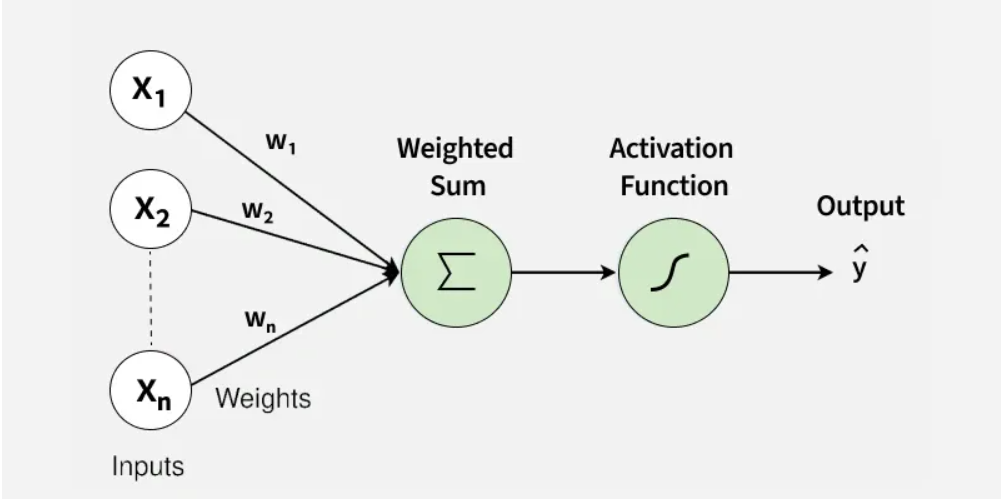
\includegraphics[width=0.8\linewidth]{images/perceptron.png}
    \caption{Perceptron}
    \label{fig:placeholder}
\end{figure}
\subsection{Forward Propagation}
For any layer l , we denote the output of previous layers as $a^{[l-1]}$, weight vector as $W^{[l]}$ and bias as $b^{[l]}$, the intermediate calculation $Z^{[l]} = W^{T[l]}a^{[l-1]} + b^{[l]}$, and the final output of this layer is $a^{[L]} = g^{[L]}(Z^{[L]})$ where $g^{[L]}$ is the activation function.
\begin{figure}[H]
    \centering
    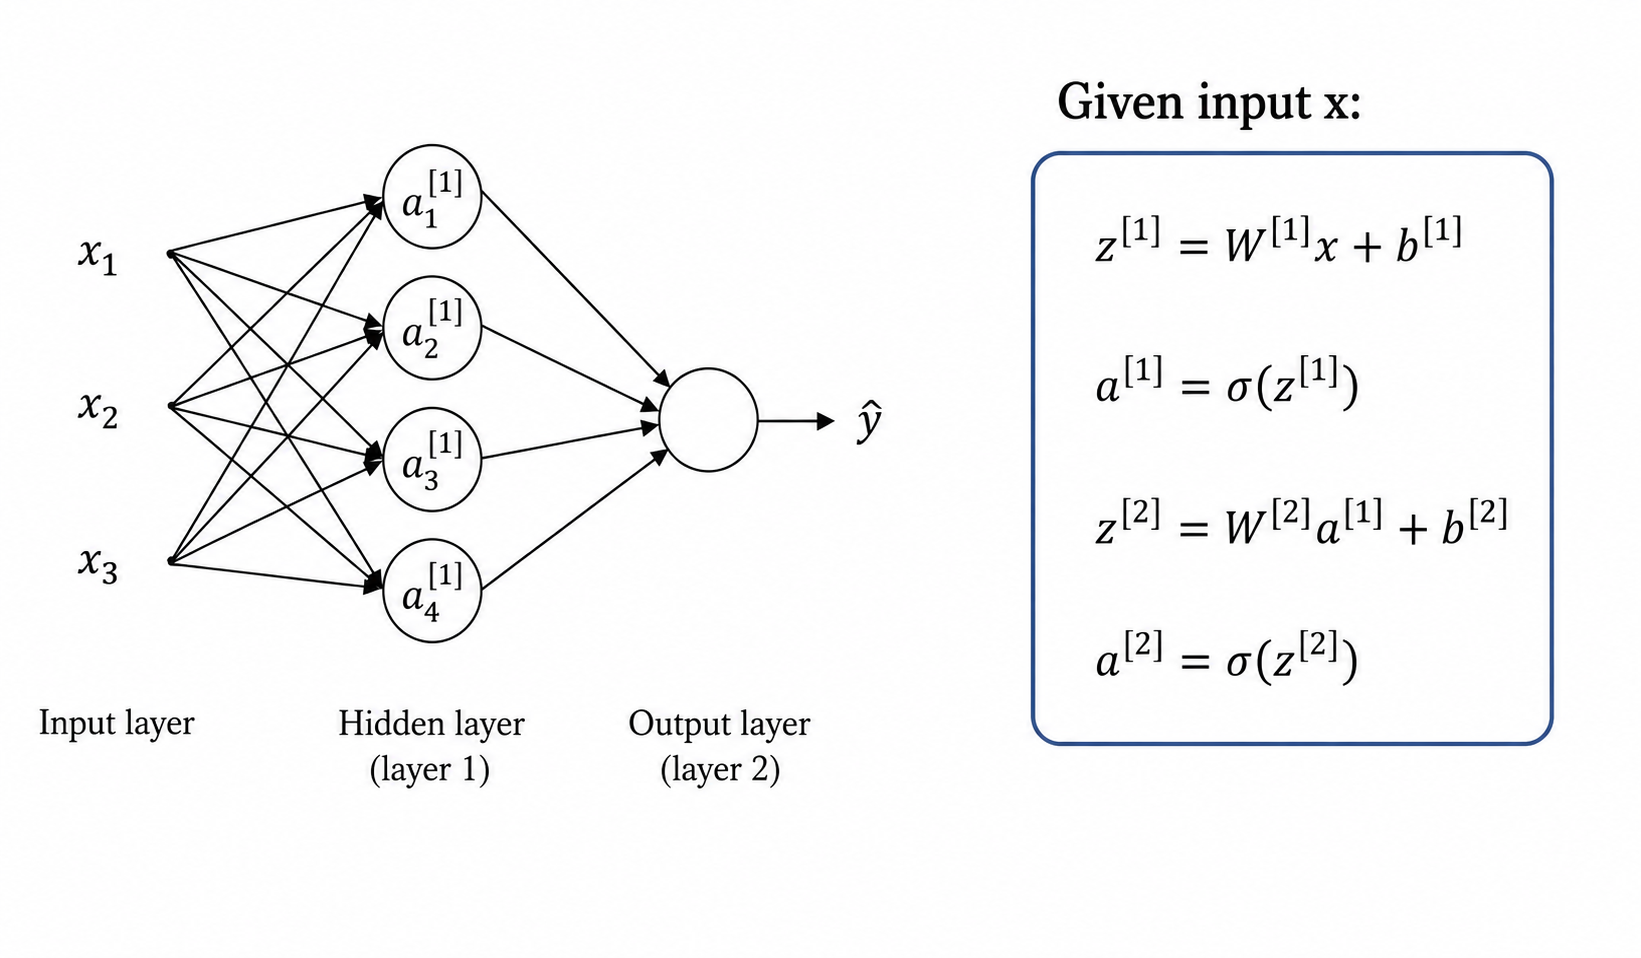
\includegraphics[width=0.5\linewidth]{images/nn.png}
    \caption{}
    \label{fig:placeholder}
\end{figure}
\subsection{Activation Functions:}
We have various options to choose from:
\subsubsection{Sigmoid Activation function}

$\sigma(x) = \frac{1}{1+e^{-x}}$. This is one of the most famous and well known activation function. In practice sigmoid function is mainly used at the last layer when we want to do binary classification(since in that case we would want our prediction to be between 0 and 1), apart from that the sigmoid activation function is rarely used.
\begin{figure}[ht]
\centering
\begin{tikzpicture}
\begin{axis}[
    axis lines=middle,
    xlabel={$x$},
    ylabel={$y$},
    domain=-6:6,
    samples=100,
    xmin=-6, xmax=6,
    ymin=0, ymax=1.2,
]
    \addplot[thick] {1/(1+exp(-x))};
\end{axis}
\end{tikzpicture}
\end{figure}
\subsubsection{Tanh activation function}
$tanh(z) = \frac{e^{z}-e^{-z}}{e^{z}+e^{-z}}$. The tanh activation function is almost always superior to the sigmoid activation function and hence this is used much more commonly that the sigmoid activation function. One downside of both tanh activation function and sigmoid activation function is that they have a almost zero slope when x is very large in magnitude which may make learning during gradient descent quite slow. To combat this we have another activation function which does not have this issue, which is the ReLU activation function.  
\begin{figure}[ht]
\centering
\begin{tikzpicture}
\begin{axis}[
    axis lines=middle,
    xlabel={$x$},
    ylabel={$y$},
    domain=-6:6,
    samples=100,
    xmin=-6, xmax=6,
    ymin=-1.2, ymax=1.2,
]
    \addplot[thick] {(exp(x)-exp(-x))/(exp(x)+exp(-x))};
\end{axis}
\end{tikzpicture}
\end{figure}
\subsubsection{ReLU activation function}
$a = max(0,x)$ , this is a great activation function which doesn't have the issue of vanishing slope , while also being able to provide non-linearity. This is the go to choice of activation function in the hidden layers.
\begin{figure}[ht]
\centering
\begin{tikzpicture}
\begin{axis}[
    axis lines=middle,
    xlabel={$x$},
    ylabel={$y$},
    domain=-6:6,
    samples=100,
    xmin=-6, xmax=6,
    ymin=-1.2, ymax=1.2,
]
    \addplot[thick] {max(0,x)};
\end{axis}
\end{tikzpicture}
\end{figure}
\subsubsection{Leaky ReLU}
This is another variation of ReLU which provides non zero gradient even for negative values. This may provide better results in certain contexts.\\ 
$a = max(0.01x,x)$ 
\begin{figure}[H] 
\centering
\begin{tikzpicture}
\begin{axis}[
    axis lines=middle,
    xlabel={$x$},
    ylabel={$y$},
    domain=-6:6,
    samples=100,
    xmin=-6, xmax=6,
    ymin=-1.2, ymax=1.2,
]
    \addplot[thick] {max(x/100,x)};
\end{axis}
\end{tikzpicture}
\end{figure}
\subsubsection{Loss Function}
Loss function is our way of telling the network which quantity it needs to minimize, or in other words how far away it's predictions were from the actual answer compared to the prediction. \\ 
Let $\hat{Y}$ be the output of the neural network and let $Y$ be the actual answer. \\ 
One way we can define is the \textbf{Mean Squared Error}
$\mathcal{L}(\hat{Y},Y) = \frac{(\hat{Y}-Y)^{2}}{2}$ \\ . 
One problem with this loss function is that it provides non-convex optimization process when we try to do gradient descent in problems like logistic regression. This gives us wrong results because we may end up in a local minima rather than a global minima. A better Loss function is the
\textbf{Cross Entropy} method. $\mathcal{L}(\hat{Y},Y) = -(Ylog(\hat{Y})+(1-Y)log(1-\hat{Y}))$ this function provides much better results for doing gradient descent. \\ 
\\ 
Loss function that we defined was how far a single prediction was from the actual answer. Because we have many training examples, the actual quantity that we minimize is the \textbf{cost} function. \\ 
$J(w,b) = \frac{1}{m}\sum_{i=1}^{m} L(\hat{y^{(i)}},y^{(i)})$ which is the average of loss function for all m training examples.
\subsubsection{Backpropagation and Chain Rule}
To train the neural network we need to minimize the cost function , as we say J is a function of w and b, hence this is an optimization problem where we need to update w and b such that J is minimzed. This can be achieved with an algorithm called \textbf{Gradient Descent}. In this algorithm we take the input and pass it through the neural network to get the output $\hat{Y}$, then we calculate the gradient of Cost function($J(w,b)$ ) with respect to W and b seperately and we update W and b until the values converge. 
\begin{lstlisting}
    while !convergence:
        (*@ $W = W - \alpha \frac{\partial J(W,b)}{\partial W}$@*)
        (*@ $b = b - \alpha \frac{\partial J(W,b)}{\partial b}$@*)
\end{lstlisting}
The process of calculating the gradients in a neural network requires us to move backwards(this directly from chain rule) from the last layer, i.e. we first calculate the gradients of the last layer then the second last layer and so on. 
Suppose we take the example with one layer,then the formulas are:
\begin{itemize}
    \item Forward Pass (for one hidden layer):
    \[
    z = W_1x + b_1,\qquad
    h = \sigma(z),\qquad
    y = W_2h + b_2
    \]

    \item Backpropagation (Chain Rule):
    \[
    \frac{\partial J}{\partial W_2}
    =
    \frac{\partial J}{\partial y}
    \cdot
    \frac{\partial y}{\partial W_2}
    \]

    \[
    \frac{\partial J}{\partial W_1}
    =
    \frac{\partial J}{\partial y}
    \cdot
    \frac{\partial y}{\partial h}
    \cdot
    \frac{\partial h}{\partial z}
    \cdot
    \frac{\partial z}{\partial W_1}
    \]

    \item Gradient Descent Update:
    \[
    W = W - \eta \frac{\partial J}{\partial W}
    \]
\end{itemize}
\subsection{Gradient Descent}
\begin{figure}[H]
    \centering
    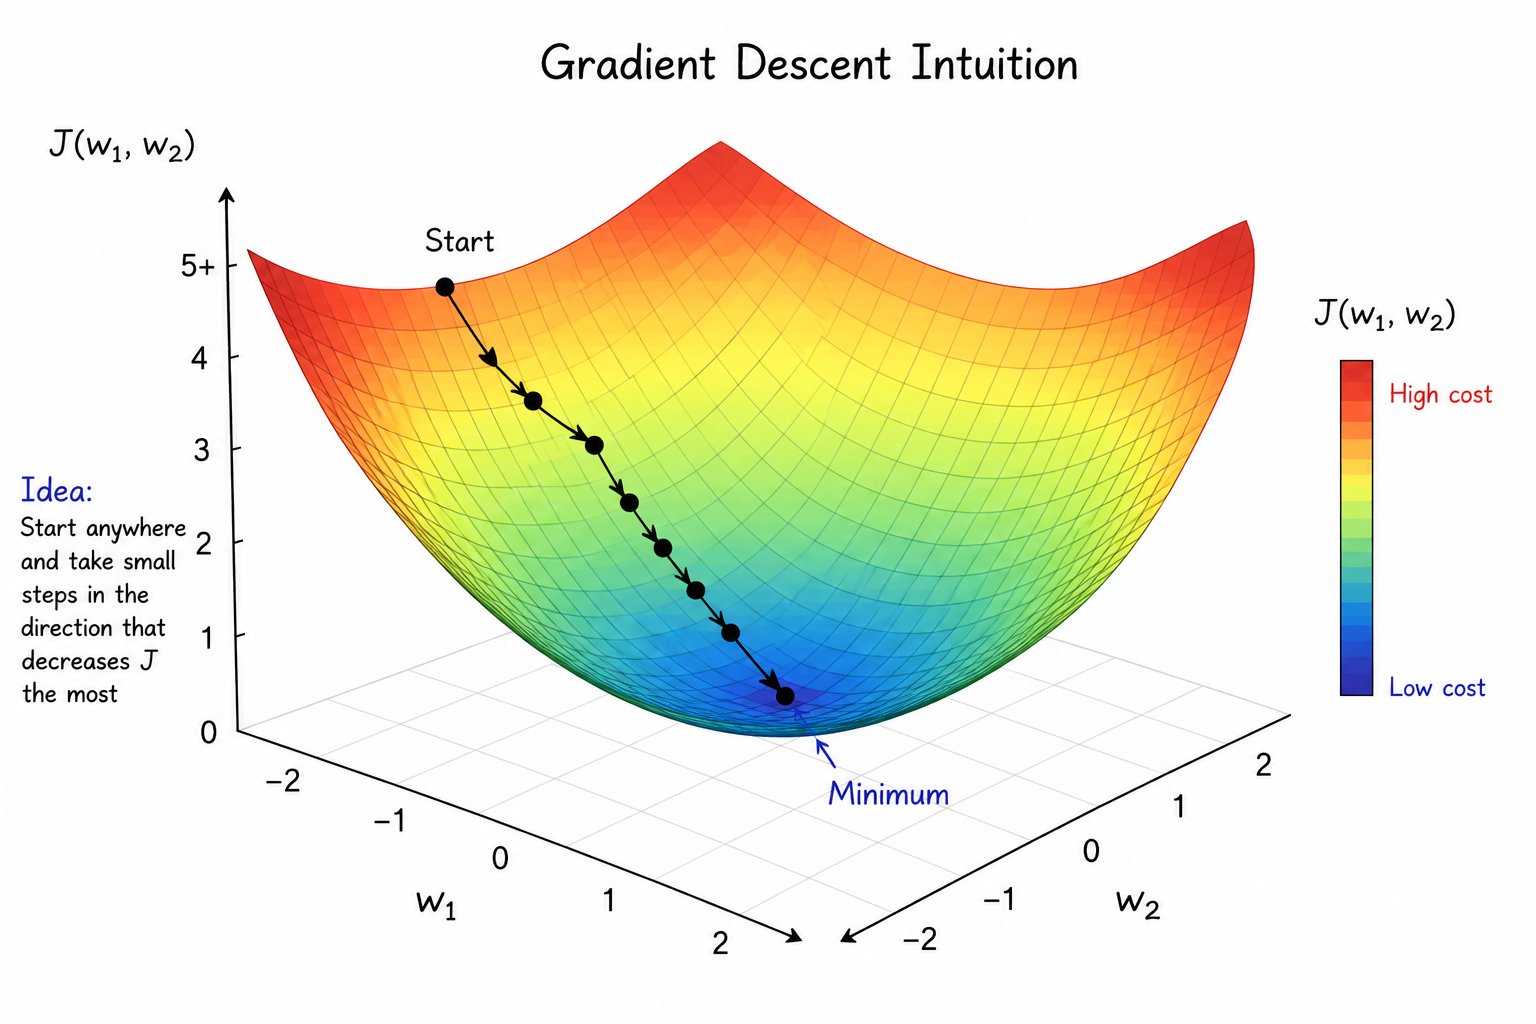
\includegraphics[width=0.5\linewidth]{images/gradi.png}
    \caption{Gradient Descent}
    \label{fig:placeholder}
\end{figure}
The reason why this works is the partial derivative is exactly along the steepest descent.
%code of section 2, make appr
\section{Week2}
\subsection{Deep vs Shallow Neural Network}
\begin{table}[H]
\centering
\caption{Comparison Between Shallow and Deep Neural Networks}
\label{tab:nn_comparison}
\vspace{0.5em}
\begin{tabular}{lp{6cm}p{6cm}}
\toprule
\textbf{Feature} & \textbf{Shallow Neural Networks} & \textbf{Deep Neural Networks} \\ \midrule
\textbf{Structure} & Neural Network will fewer number of layers. & Neural network with many layers (multiple hidden layers, this number has even exceeded billions in last few years!). \\ \addlinespace
\textbf{Complexity} & Complexity is low. & Complexity is high. \\ \addlinespace
\textbf{Capacity} & less learning capacity. & Higher learning capacity. \\ \addlinespace
\textbf{Overfitting} & Lower risk of overfitting. & Higher risk of overfitting. \\ \addlinespace
\textbf{Data Requirement} & Requires less data. & Requires huge amounts of data \\ \addlinespace
\textbf{Computation} & Requires less computational resources. & Requires more computational resources (e.g., GPUs). \\ \addlinespace
\textbf{Examples} & Single-layer Perceptron, Logistic Regression. & Convolutional Neural Networks (CNNs), Recurrent Neural Networks (RNNs). \\ \bottomrule
\end{tabular}
\end{table}
\subsection{Weight Initialization techniques}
This part is much more important than it initially seems. Let's assume that we initialize the weights and biases to zero. This leads to the problem that the weight graph will always remain symmetric no matter what,which will lead to the neural network not learning the actual function. \\ 
The better way for us is to initialize is to initialize the weights to small random values and since we have introduced randomness in weights, we can safely assign biases to zeros. // 
\begin{lstlisting}[language=Python]
W[1] = np.random.randn((2,2)) * 0.01
b[1] = np.zeros((2,1))
\end{lstlisting}
Why have we multiplied it with 0.01 ? Remember if we were using sigmoid or tanh activating function, they have high slopes near zero hence learning rate will be fast when we initialize out values to near zero. \\ 
This is the most basic way of initializing weights. Due to the problem of vanishing and exploding gradients, there are better ways to initilize weights and biases. \\ 
\begin{lstlisting}
    W[l] = np.random.randn(shape) * np.sqrt(2/n[l-1])
\end{lstlisting}
This initialization method was proposed by the authors in [He et al Diving Deep into Rectifiers] . This works best when our activation function is the ReLU activation function. \\ 
There are other methods as well such as Xavier's Initialization which works best when we use the tanh activation function. \\ 
\begin{lstlisting}
    W[l] = np.random.randn(shape)*np.sqrt(1/n[l-1])
\end{lstlisting}
There are some other variations as well where we use 
\begin{lstlisting}
    W[l] = np.random.randn(shape)*np.sqrt(2/(n[l-1]+n[l]))
\end{lstlisting}
\subsection{Vanishing and Exploding Gradients}
As the name suggests this problem happens when either the gradient(during the gradient calcualtion part during backpropagation) either vanishes(becomes extremely small i.e. -> 0) or explodes(becomes extremely large i.e. -> $\infty$. To gain an intuition as to why this happens let us visualize a very basic and simple deep neural network with lot's of layers and the linear activation function $g(z)=z$ \\ 
The output in this case is \\ 
$\hat{Y} = W^{[L]}W^{[L-1]}W^{[L-2]}\dots W^{[2]}W^{[1]}$
Now Imagine W is a diagonal matrix with entries slighly more than $I$ then Y as well as the gradient will explode, and if it is slightly less than $I$ then Y as well as the gradient will vanish. To solve this problem from happening in deep neural networks we use different types of weight initialization techniques such as He's Initialization or Xavier's initialization.
\subsection{Stochastic Gradient Descent and Mini-batch Gradient Descent}
What we did till now was Batch Gradient descent, i.e. we used all our data at once (forward and backward propagation). However there is a different way of training as well, what we can do is divide our whole batch of data in mini-batches of some size say k. Then we can individually train on these batches(i.e. apply full gradient descent on these mini batches one after another).
This leads to the gradient process to look like this: 
\begin{figure}[H]
    \centering
    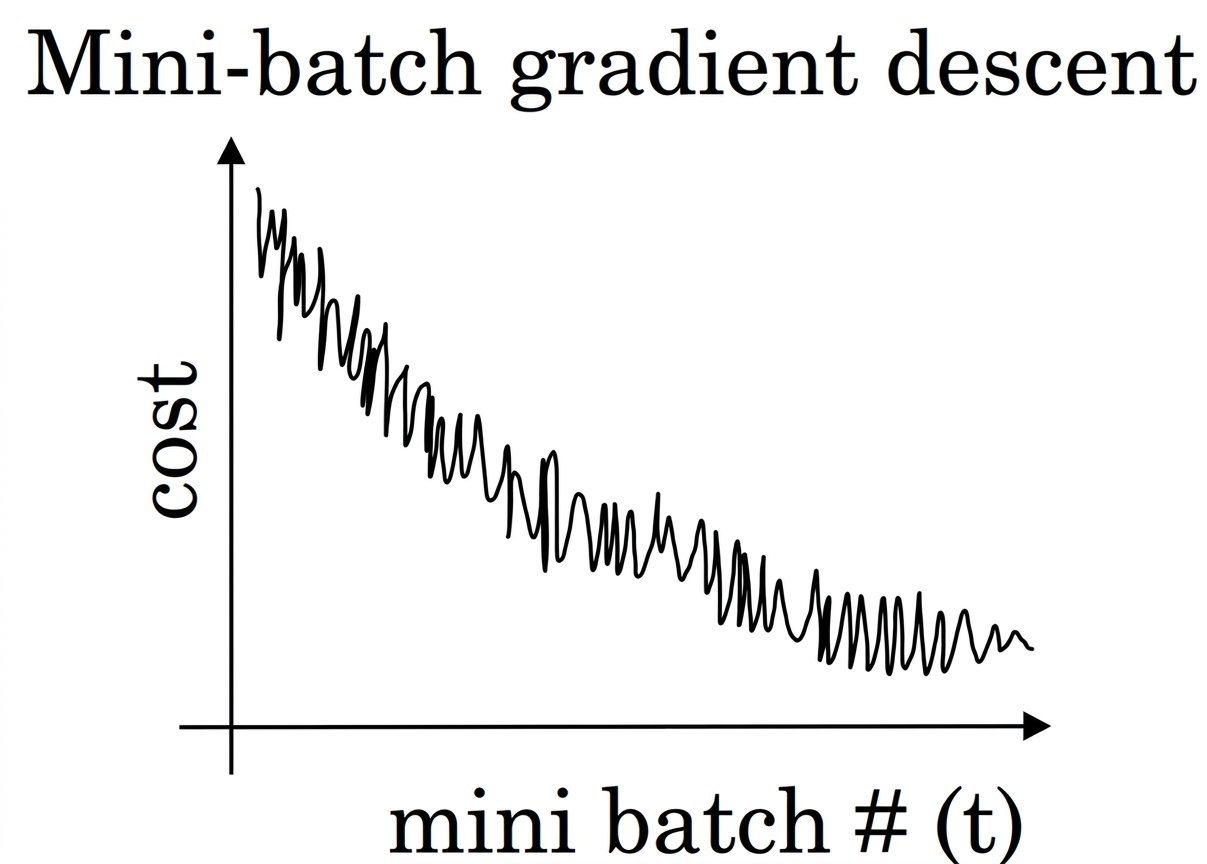
\includegraphics[width=0.5\linewidth]{images/grad.png}
    \caption{}
    \label{fig:placeholder}
\end{figure}
k is a hyperparameter, the case with k = m is called the batch gradient descent , when k is between 1 and m it is called the mini-batch gradient descent and when k = 1 we call it the stochastic gradient descent. \\
If we use stochastic gradient descent we loose the speed gained due to vectorization, if we use batch gradient descent that is too long per iteration. The ideal value of k is generally between 1 and m. In practice the values of k is generally taken to be powers of 2 such as 64,128,256 etc, there are various reasons for this(it might be realted to computer architechure). 
\begin{figure}[H]
    \centering
    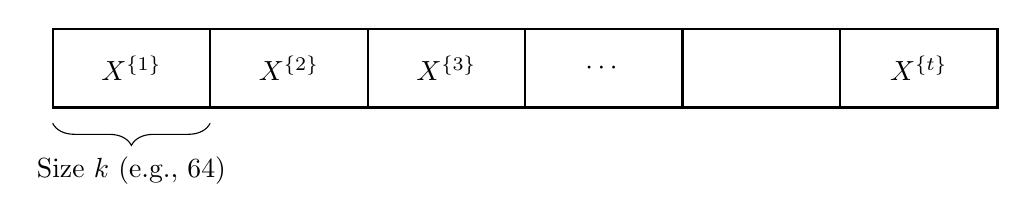
\begin{tikzpicture}

        % Entire dataset
        \draw[thick] (0,0) rectangle (12,1);

        % Split into mini-batches
        \foreach \x in {2,4,6,8,10}
            \draw[thick] (\x,0) -- (\x,1);

        % Labels
        \node at (1,0.5) {$X^{\{1\}}$};
        \node at (3,0.5) {$X^{\{2\}}$};
        \node at (5,0.5) {$X^{\{3\}}$};
        \node at (7,0.5) {$\cdots$};
        \node at (11,0.5) {$X^{\{t\}}$};

        % Bracket indicating mini-batch size
        \draw[decorate,decoration={brace,mirror,amplitude=8pt}]
            (0,-0.2) -- (2,-0.2)
            node[midway,yshift=-0.6cm] {Size \(k\) (e.g., 64)};

    \end{tikzpicture}

    \caption{The training set divided into mini-batches of size \(k\).}
\end{figure}
\subsection{Gradient Descent with momentum}
Here we estimate value of dW and db (dW is the partial derivative of cost function with respect to W) using \textbf{exponentially weighted averages} . More concretely 
\begin{lstlisting}
    for iteration t: 
        Compute dW, db on current mini batch and then use EMA(exponentially moving average) 
        (*@$V_{dW} = \beta V_{dW} + (1 - \beta)dW$@*)
        (*@$V_{db} = \beta V_{db} + (1 - \beta)db$@*)
\end{lstlisting}
Here we have introduced yet another hyperparameter($\beta$) typically set to 0.9.
\subsection{RMS prop}
This is in many ways quite similar to momentum. Here the formulas are a bit different. \\
\begin{lstlisting}
    for iteration t: 
        Compute dW, db on current mini batch and then use EMA(exponentially moving average) 
        (*@$S_{dW} = \beta S_{dW} + (1 - \beta)dW^2$@*)
        (*@$S_{db} = \beta S_{db} + (1 - \beta)db^2$@*)
\end{lstlisting} 
then we update \\ 
$W = W - \frac{\alpha dW}{\sqrt{S_{dW}+\epsilon}}$ \\ 
$b = b - \frac{\alpha db}{\sqrt{S_{db}+\epsilon}}$ \\
here $\beta$ is typically set to 0.999 and $\epsilon$ is typically set to $10^{-8}$
\subsection{Adam's optimization algorithm}
Adam's optimization is one of the popular and go to optimization algorithm that people use. Adam is just a combination of RMSprop and Momentum, along with bias correction factor.
\begin{lstlisting}
    for iteration t: 
        Compute dW, db on current mini batch and then use EMA(exponentially moving average) 
        (*@$V_{dW} = \beta V_{dW} + (1 - \beta_1)dW$@*)
        (*@$V_{db} = \beta V_{db} + (1 - \beta_1)db$@*)
        (*@$S_{dW} = \beta S_{dW} + (1 - \beta_2)dW^2$@*)
        (*@$S_{db} = \beta S_{db} + (1 - \beta_2)db^2$@*)
        (*@ $V_{dW} /= (1-(\beta_1)^{t})$@*)
        (*@ $V_{db} /= (1-(\beta_1)^{t})$@*)
        (*@ $S_{dW} /= (1-(\beta_2)^{t})$@*)
        (*@ $S_{db} /= (1-(\beta_2)^{t})$@*)
        (*@ $W = W - \frac{\alpha V_{dW}}{\sqrt{S_{dW}+\epsilon}}$ @*)
        (*@ $b = b - \frac{\alpha V_{db}}{\sqrt{S_{db}+\epsilon}}$ @*)
\end{lstlisting} 
Here the standard values of $\beta_1$, $\beta_2$, $\epsilon$ are same as used in RMSprop and momentum(i.e. 0.9,0.999,$10^{-8}$ respectively)
\subsection{Bias-Variance Tradeoff}
Machine Learning is a very iterative process. We first train our model on data known as the training set. We then check how good the model is using the dev set. If the results are satisfactory, we are done. Otherwise, we make suitable changes to the model and evaluate it again. We keep repeating this process until we obtain results that we are happy with. Finally, before deployment, we perform one last evaluation using the test set. It is completely possible for a team to not have a separate test set and only maintain training and dev sets. In the older days, a common split was $60/20/20$ for the training, dev, and test sets. The primary reason for this was the lack of data. In many modern applications, however, data is abundant, and hence splits such as $98/1/1$ have become quite common. \begin{figure}[h]
    \centering
    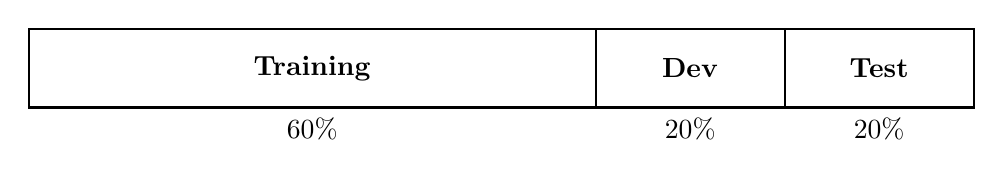
\begin{tikzpicture}

        % Outer bar
        \draw[thick] (0,0) rectangle (12,1);

        % 60/20/20 split
        \draw[thick] (7.2,0) -- (7.2,1);
        \draw[thick] (9.6,0) -- (9.6,1);

        % Labels
        \node at (3.6,0.5) {\textbf{Training}};
        \node at (8.4,0.5) {\textbf{Dev}};
        \node at (10.8,0.5) {\textbf{Test}};

        % Percentages
        \node[below] at (3.6,0) {60\%};
        \node[below] at (8.4,0) {20\%};
        \node[below] at (10.8,0) {20\%};

    \end{tikzpicture}

    \caption{Traditional train--dev--test split. Modern large-scale datasets may use much smaller dev and test sets (for example, 98/1/1), but such splits are not shown to scale here for clarity.}
\end{figure} For comparison, traditional datasets often used a $60/20/20$ split, whereas modern large-scale datasets may use distributions such as $98/1/1$.
We can come across many situations after training on the training set and evaluating on the dev set. Based on the observed errors, we have some useful thumb rules for diagnosing what might be going wrong. A low training error but a high dev error means that the model has overfitted the training data. This is known as high variance. A high training error means that the model has underfitted and is unable to capture the underlying patterns present in the data. This is known as high bias. There are four common situations that we may encounter: \begin{table}[h] \centering \caption{Diagnosing bias and variance from training and dev errors.} \begin{tabular}{lll} \toprule Training Error & Dev Error & Interpretation \\ \midrule Low & Low & Low bias and low variance.  \\ High & Similar to training error & High bias (underfitting). \\ Low & Much higher than training error & High variance (overfitting).  \\ High & Much higher than training error & High bias and high variance.  \\ \bottomrule \end{tabular} \end{table} Some example values are shown below: \begin{table}[h] \centering \caption{Example error values and their interpretation.} \begin{tabular}{ccc} \toprule Train Error & Dev Error & Diagnosis \\ \midrule $0.5\%$ & $1\%$ & Low bias and low variance \\ $15\%$ & $16\%$ & High bias \\ $1\%$ & $11\%$ & High variance \\ $15\%$ & $30\%$ & High bias and high variance \\ \bottomrule \end{tabular} \end{table} Historically, this was referred to as the bias--variance tradeoff. Since bias corresponds to underfitting and variance corresponds to overfitting, people often observed that reducing one increased the other. However, modern machine learning has progressed enough that we now have techniques that can reduce bias without significantly affecting variance, and techniques that can reduce variance without significantly affecting bias. As a result, the tradeoff is not as strict as it used to be.
\begin{tikzpicture}[
    node distance=1.8cm and 3cm,
    box/.style={
        draw,
        rectangle,
        minimum width=3cm,
        minimum height=1cm,
        align=center
    },
    decision/.style={
        align=center
    },
    arrow/.style={
        -{Latex[length=3mm]},
        thick
    }
]

% Left side
\node[decision] (bias) {\textbf{High Bias?}\\(Training set performance)};

\node[decision, below=2cm of bias] (variance) {\textbf{High Variance?}\\(Dev set performance)};

\node[below=1.8cm of variance] (done) {\Large Done};

% Right side
\node[box, right=4cm of bias] (bigger) {Bigger Network};

\node[below=0.4cm of bigger, align=left] (biasnotes)
{
$\rightarrow$ Train longer\\
( NN architecture search )
};

\node[box, right=4cm of variance] (data) {More Data};

\node[below=0.4cm of data, align=left] (varnotes)
{
$\rightarrow$ Regularization\\
( NN architecture search )
};

% Arrows
\draw[arrow] (bias) -- node[above] {Y} (bigger);

\draw[arrow] (bias) -- node[left] {N} (variance);

\draw[arrow] (variance) -- node[above] {Y} (data);

\draw[arrow] (variance) -- node[left] {N} (done);

% Loop back
\draw[arrow]
    ([xshift=1cm]bigger.east)
    -- ++(2,0)
    -- ++(0,-5)
    -- ([xshift=1cm]data.east);

\draw[arrow]
    ([xshift=3cm]data.east)
    -- ++(1,0)
    -- ++(0,7)
    -- ([yshift=0.5cm]bias.north);


\end{tikzpicture}
\subsection{PyTorch Basics}

PyTorch is one of the most widely used deep learning frameworks. 

\subsubsection{Tensors}
Tensors are the fundamental data structures in PyTorch. They are similar to NumPy arrays but can also be efficiently executed on GPUs.

\begin{lstlisting}[language=Python]
import torch

x = torch.tensor([[1., 2.],
                  [3., 4.]])

y = torch.randn(2, 2)

z = x + y
print(z)
\end{lstlisting}

\subsubsection{Autograd}
PyTorch automatically computes gradients using computation graphs.

\begin{lstlisting}[language=Python]
x = torch.tensor(2.0, requires_grad=True)

y = x**2 + 3*x + 1

y.backward()

print(x.grad)   # dy/dx = 2x + 3 = 7
\end{lstlisting}

\subsubsection{Building Models using \texttt{nn.Module}}
Neural networks in PyTorch are typically defined by inheriting from \texttt{nn.Module}. The forward method specifies the computation performed during the forward pass.

\begin{lstlisting}[language=Python]
import torch.nn as nn

class SimpleNN(nn.Module):
    def __init__(self):
        super().__init__()
        self.fc1 = nn.Linear(4, 8)
        self.fc2 = nn.Linear(8, 1)

    def forward(self, x):
        x = torch.relu(self.fc1(x))
        return self.fc2(x)

model = SimpleNN()
print(model)
\end{lstlisting}

\section{Week 3:}
\subsection{Regularization Techniques}
To solve the problem of High Variance one of the techniques is to use regularization. \\
First we define the Frobenius norm of a matrix as 
$||W^{[L]}||^{2}_{2} = \sum_{i=1}^{n^{[L]}} \sum_{j=1}^{n^{[L-1]}}(w_{i,j}^{[L]})^2$. One of the most popular regularizing techniques is the \textbf{L2 regularizing method}. Here we add an extra term in the cost function. \\ 
$J(W^{[1]},b^{[1]},\dots,W^{[L]},b^{[L]}) = \frac{1}{m} \sum_{i=1}^{m}\mathcal{L}(\hat{y}^{(i)},y^{(i)}) + \frac{\lambda}{2m} \sum_{l=1}^{L} ||W^{[l]}||^{2}_{F}$. This has a regularizing effect as it punishes the network for putting too much weight on neuron rather than making them smaller and distributing them more. 
We can \textbf{L1 regularization} as well where simply we use the norm directly without squaring it, we can use either but in practice it is found that L2 regularization seems to work better. 
\subsection{Dropout Regularization}
This achieves a similar result to $L2$ regularization. In Dropout regularization or "inverted dropout" during training time we random "shut off" few neurons i.e. we pretend as if they are not there. We do this with probability keep\_prob which is another hyperparameter. 
Say we apply dropout at layer 3 
\begin{lstlisting}
    d3 = np.random.randn(a3.shape[0],a3.shape[1])<keep_prob
    a3 = np.multiply(a3,d3)
    a3 /= keep_prob #We do this step to ensure that expected value of a3 remains the same
\end{lstlisting}
During the testing time however we do not do dropout and apply forward propagation normally. \\ 
The intuition behind why dropout works is that it forces the network to distribute the weight rather than putting too much weight on a single neuron(this prevents overfitting). 
\subsection{Batch Normalization}
\subsubsection{Normalizing training set}
To normalize training set we subtract the mean \\ 
$\mu =\frac{1}{m}\sum_{i=1}^{m}x^{(i)}$ and divide by the std. dev \\ 
$\sigma^2 = \frac{1}{m}\sum_{i=1}^{m}x^{(i)}**2 - \mu^2$
So we get 
$X := \frac{X-\mu}{\sigma}$ 
\\ In practice this significantly improves the gradient descent speed as it makes the contours of the cost function more spherical rather than elliptic. The following images shows why the visualization in 3D. 
\begin{figure}[H]
    \begin{subfigure}{0.45\textwidth}
        \centering
        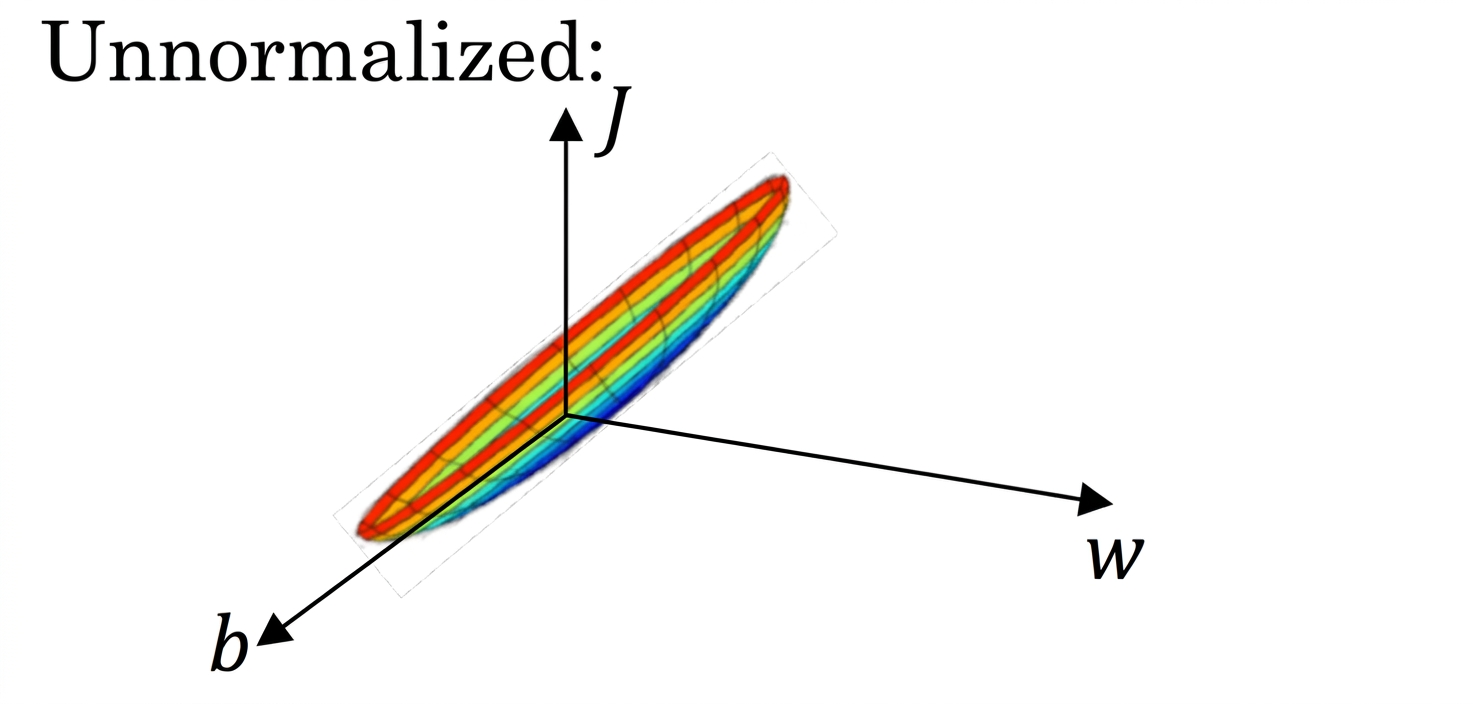
\includegraphics[width=\linewidth]{images/before.png}
        \caption{First image}
    \end{subfigure}
    \hfill
    \begin{subfigure}{0.45\textwidth}
        \centering
        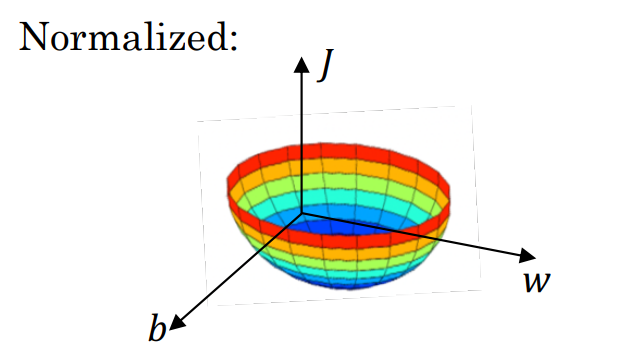
\includegraphics[width=\linewidth]{images/after.png}
        \caption{Second image}
    \end{subfigure}
\end{figure}
\subsubsection{Intermediate Value}
Given some intermediate values in the Neural Network \\ 
$Z^{[l](i)}, \dots, Z^{[l](m)}$ calculate the mean and variance and set $Z_{norm}^{i} = \frac{(Z^{(i)}-\mu)}{\sqrt{(\sigma^2+\epsilon)}}$ we add a small quantity $\epsilon = 10^{-8}$ in the bottom to avoid dividing by zero. After this we set $\tilde{z}^{i} = \gamma z_{norm}^{i} + \beta$ here $\gamma$ and $\beta$ are learnable parameters of the model(not hyperparameters!). These two quantities also determine the mean and variance of the new values. We can see than $\beta$ technically does the job of the biases hence we don't need $b^{[L]}$ anymore! \\ 
During the test time we estimate $\mu$ and $\sigma$ using exponentially weighted average(across mini batches)
\subsection{Learning Rate Scheduling}
As we approach the global minimum, it is a wise idea to reduce our learning rate (so that we don't jump over the minima), this leads us to the concept of "learning rate decay" where learning rate decays as we move across mini batches. There are many different formulas through which we can reduce the learning rate. Using an iterative process we can find which learning rate decay model works best for our particular application. \\ (epoch number means the number of mini batches we have already trained on)
$\alpha = \frac{\alpha_0}{1 + decayRate*epochnumber}$ \\ 
$\alpha = \alpha_0 * (0.95)^{epochnumber}$ \\ 
$\alpha = \alpha_0 * \frac{k}{\sqrt{epochnumber}}$ \\ 
Or we can even manually change alpha if we tuning such a big model that takes weeks or months to train. 
\section{Week 4}
\subsection{Basics of Image Classification/Computer Vision}
There are many interesting problems in the field of computer vision. These can be broadly classified as 
\begin{enumerate}
    \item Image Classification(Suppose we want to classify from a set of images if an image is a cat or not)
    \item Object Detection
    \item Neural Style Transfer
\end{enumerate}
The first question we come across is how do we give an image as an input to the neural network ?. Here's what we will do we decompose every pixel into it's constitutent colors i.e. RGB, then we get pxpx3 different numbers between say 0 and 256 no we stack these $3p^2$ numbers in a single column matrix and that becomes our input to the neural network. 
\begin{figure}[H]
    \centering
    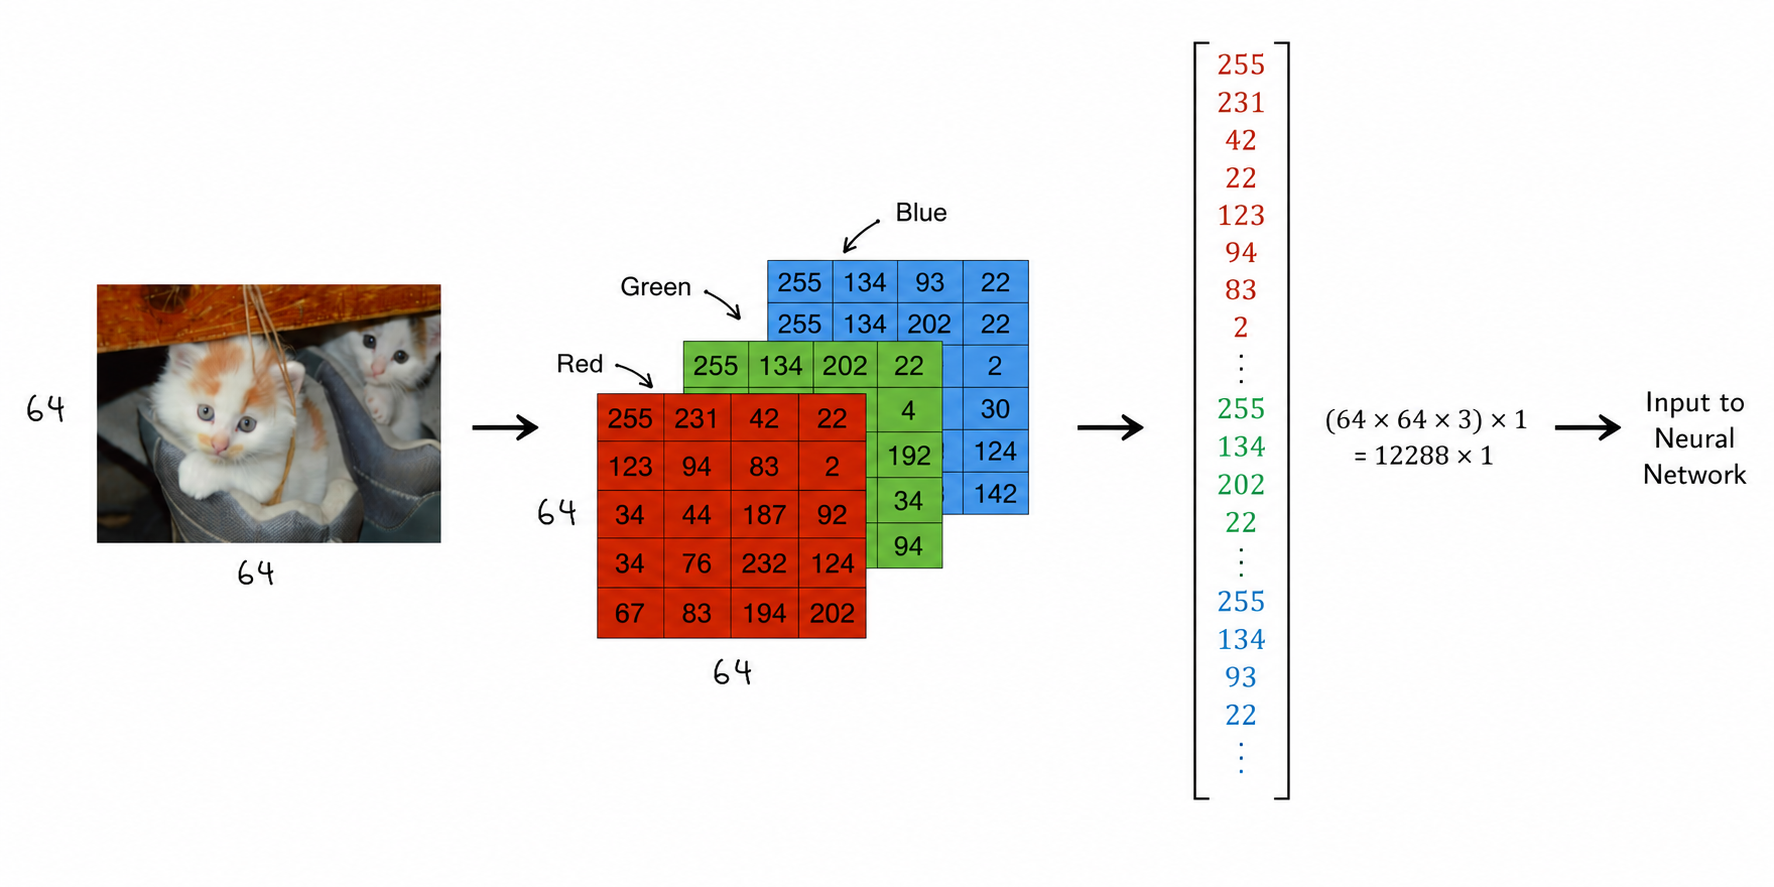
\includegraphics[width=0.5\linewidth]{images/input.png}
    \caption{Converting image into vector}
    \label{fig:placeholder}
\end{figure}
\subsection{Convolution Operator}
If we are working with a very high resolution image suppose a 1000x1000 image, and we subsequently reduce it to say 500x500 then the number of parameters required in a fully connected layer would be 1000x1000x500x500x3x3 which well above a billion parameters , which requires seemingly impossible amount of computation power. \\
This issue of very large amounts of parameters seeks us to look for another type of method. Convolution operator is one such method which works remarkably well for computer vision applications. \\
A big reason why it works remarkably well for computer vision purposes is because of \textbf{parameter sharing} which means we use the same weights again and again .Images are also very much translationally invariant which means a cat shifted by few pixels is also a cat, and this is perfectly synchronous with the convolution operation \\ 
\begin{enumerate}
    \item A small matrix called a filter (kernel) slides over the input image to extract important features.
    \item At each position, the filter performs element-wise multiplication with the image patch.
    \item The multiplied values are summed together to produce a single output value.
    \item This operation is repeated across the entire image using a defined stride.
    \item The result is a new matrix called a feature map, which highlights detected patterns.
    \item If resolution of image is nxn and size of filter is fxf then the output matrix has dimensions 
    $(n-f+1)$ x $(n-f+1)$
\end{enumerate}
\begin{figure}[H]
    \centering
    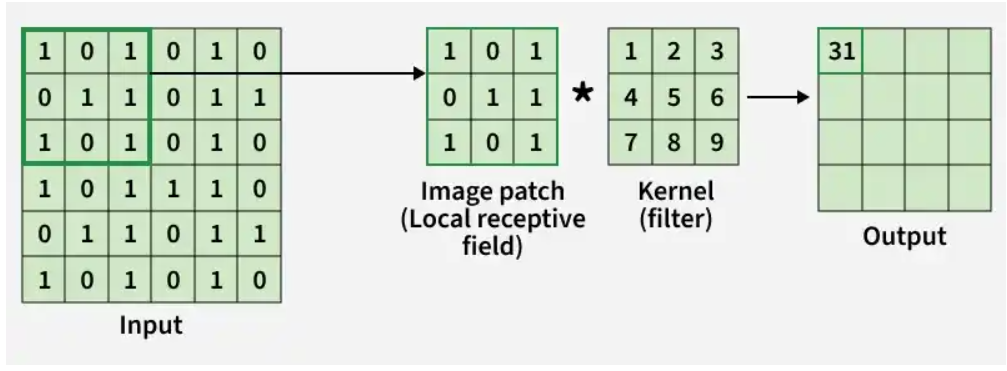
\includegraphics[width=0.5\linewidth]{images/convo.png}
    \caption{}
    \label{fig:placeholder}
\end{figure}

\begin{figure}[H]
    \centering
    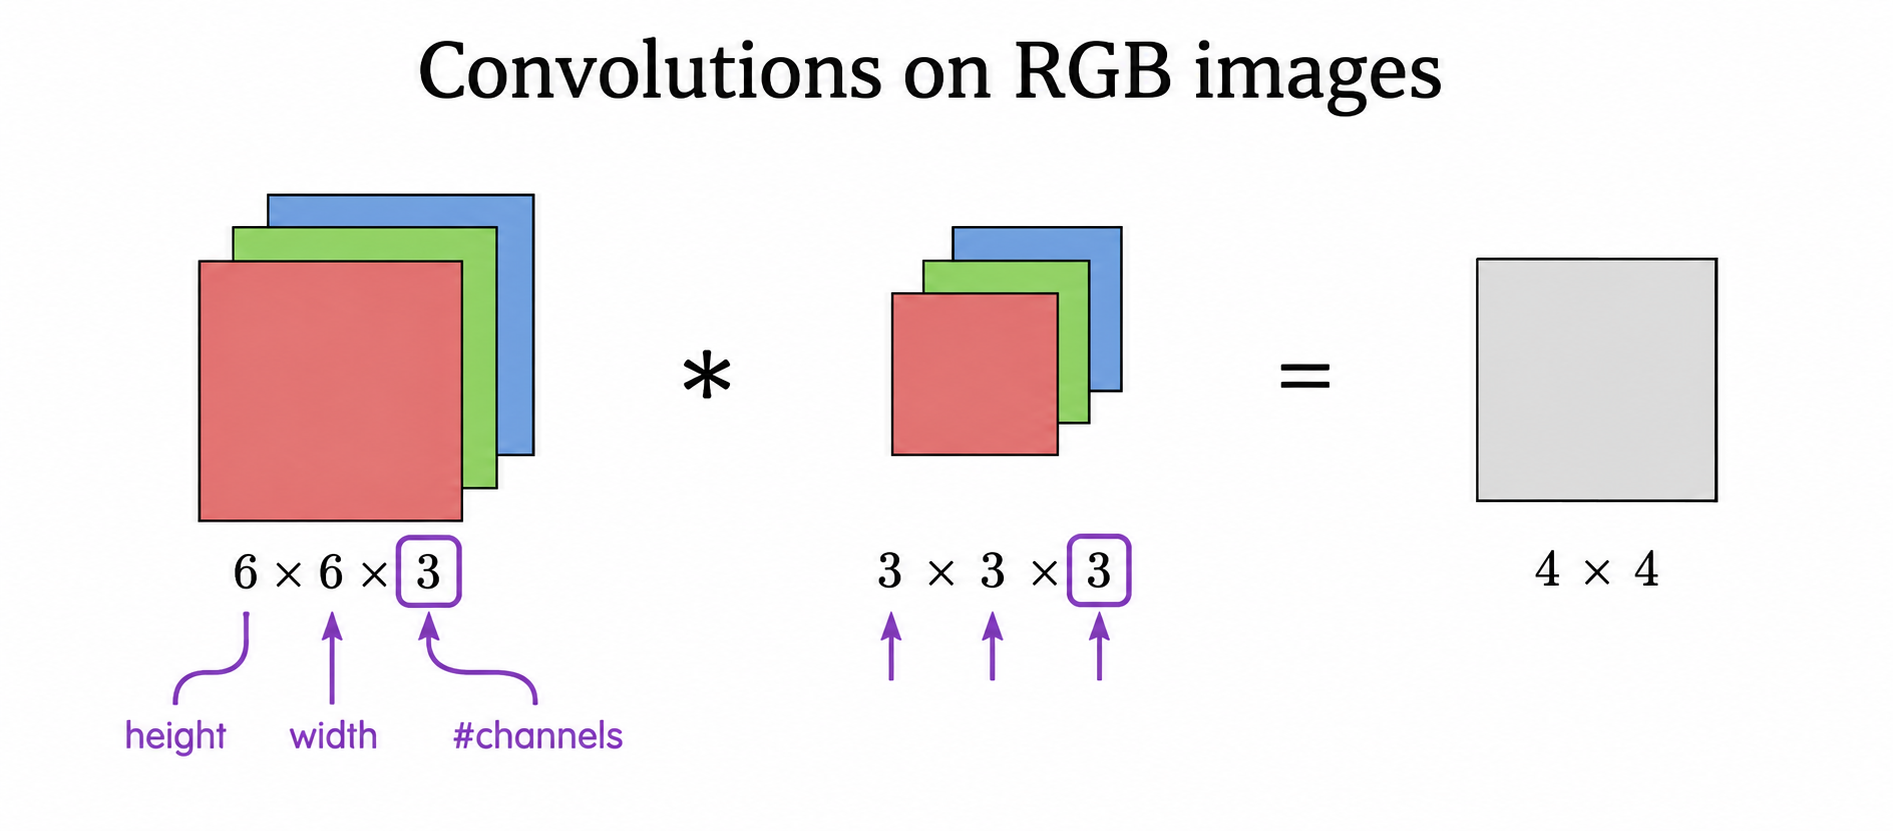
\includegraphics[width=0.7\linewidth]{images/conv.png}
    \caption{Convolution Operator}
    \label{fig:placeholder}
\end{figure}
\begin{figure}[H]
    \centering
    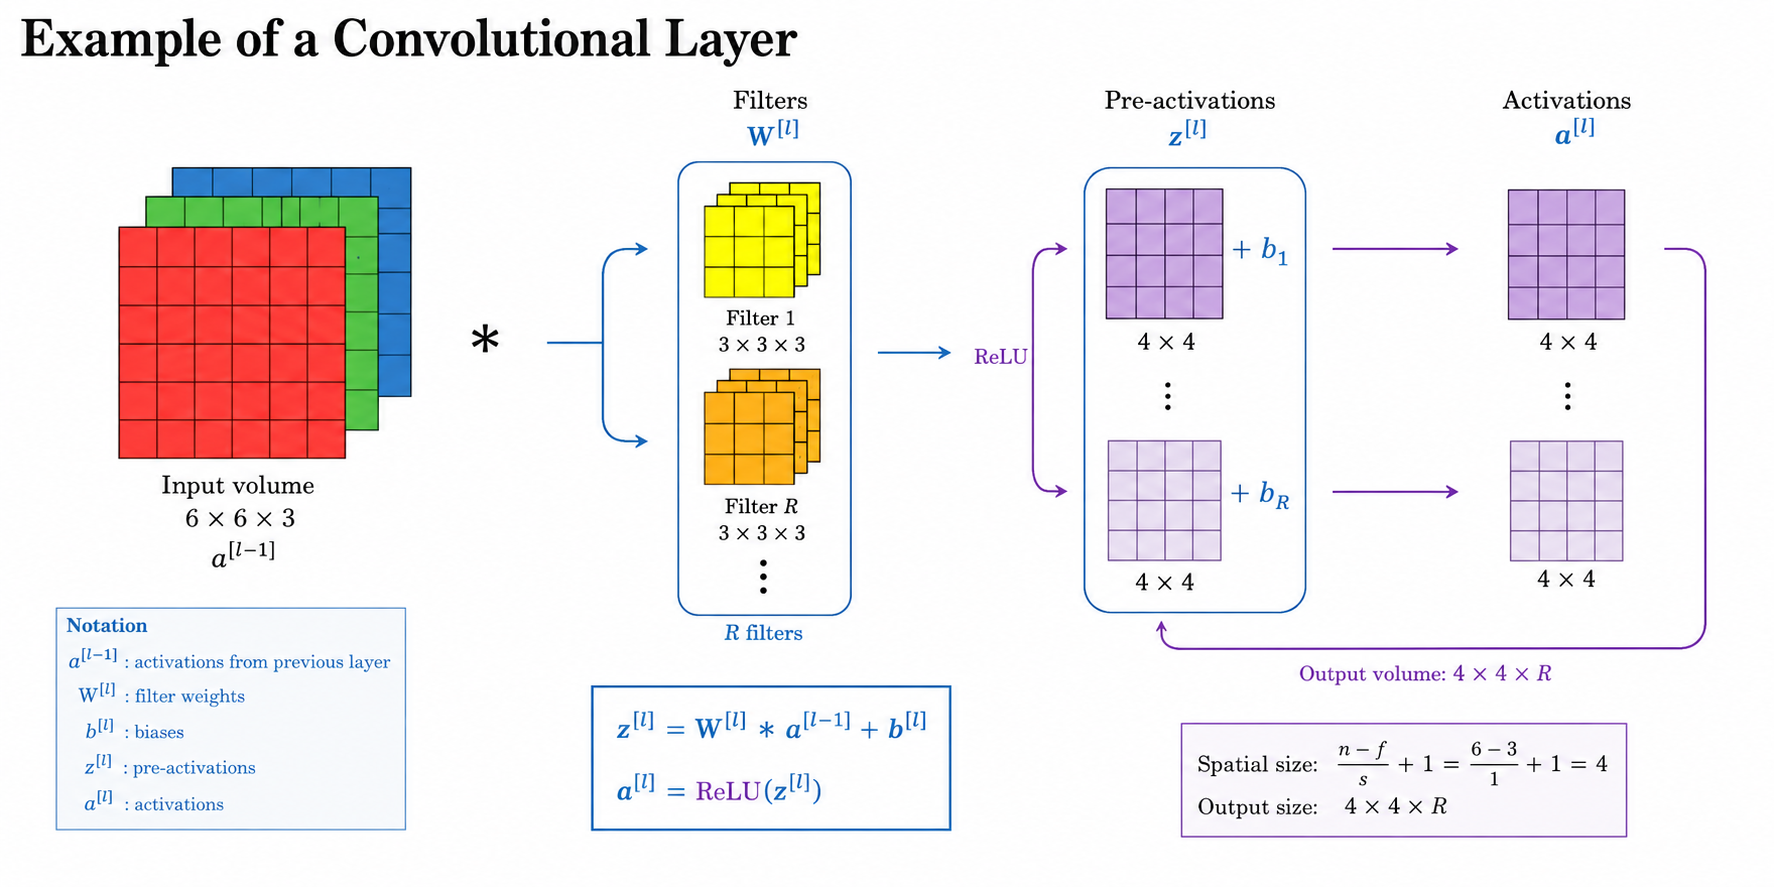
\includegraphics[width=0.9\linewidth]{images/CNN.png}
    \caption{How a Convolution layer looks like}
    \label{fig:placeholder}
\end{figure}
A convolution operator detects various features of the image, we use many convolution layers and many filters in those layers to extract various features. \\ 
For example the following filter detect a vertical edge: 
\begin{figure}[H]
    \centering
    \[
    \text{Vertical Edge Detector}
    \qquad
    \text{Sobel Filter}
    \qquad
    \text{Scharr Filter}
    \]

    \[
    \begin{bmatrix}
    1 & 0 & -1 \\
    1 & 0 & -1 \\
    1 & 0 & -1
    \end{bmatrix}
    \qquad\qquad
    \begin{bmatrix}
    1 & 0 & -1 \\
    2 & 0 & -2 \\
    1 & 0 & -1
    \end{bmatrix}
    \qquad\qquad
    \begin{bmatrix}
    3 & 0 & -3 \\
    10 & 0 & -10 \\
    3 & 0 & -3
    \end{bmatrix}
    \]

    \caption{Examples of filters used for detecting vertical edges. From left to right: a simple vertical edge detector, the Sobel operator, and the Scharr operator.}
    \label{fig:edge_filters}
\end{figure}
This is how they detect edges. 
\begin{figure}[H]
    \centering
    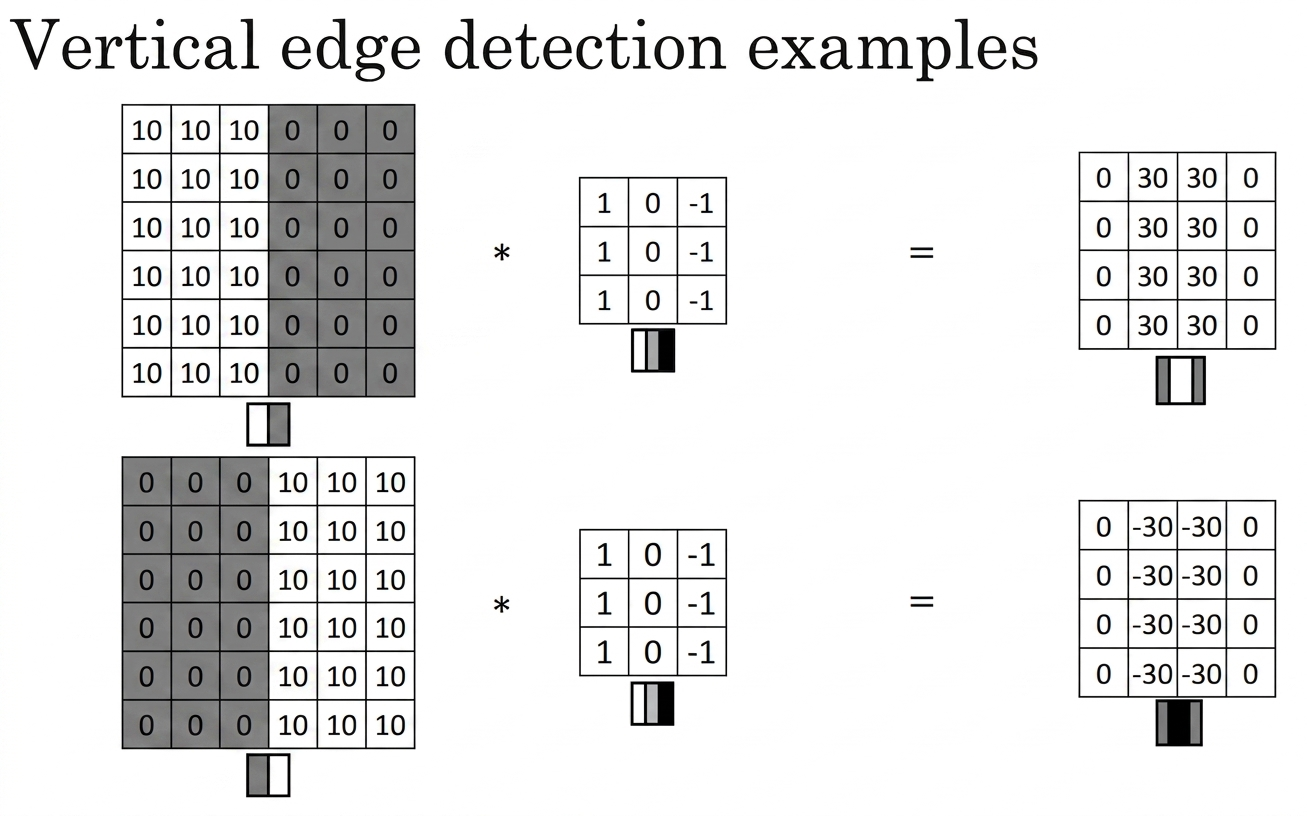
\includegraphics[width=0.5\linewidth]{images/edge.png}
    \caption{Edge Detection}
    \label{fig:placeholder}
\end{figure}
\subsubsection{Padding}
Suppose we do not want reduce the size of the image(i.e. we want to do a "same" convolution) , what we can do is pad the matrix with zero along it's border, the amount of padding is denoted by $p$. after padding we will apply a filter of size $f$ then the size of the output matrix will be $(n+2p-f+1) = n \implies p = (f-1)/2$. Even when we donot want to do a same convolution we can also do padding (p is another hyperparameter like f).
\subsubsection{Stride}
We may decide to skip some squares while sliding our filter this is denoted by $s$ i.e. the stride. The final size of the matrix when we do padding of $p$, stride of $s$ and filter of size $f$ is: \\ 
$\lceil \frac{n+2p-f}{s} + 1 \rceil$ \\
The following image explains stride visually. 
\begin{figure}
    \centering
    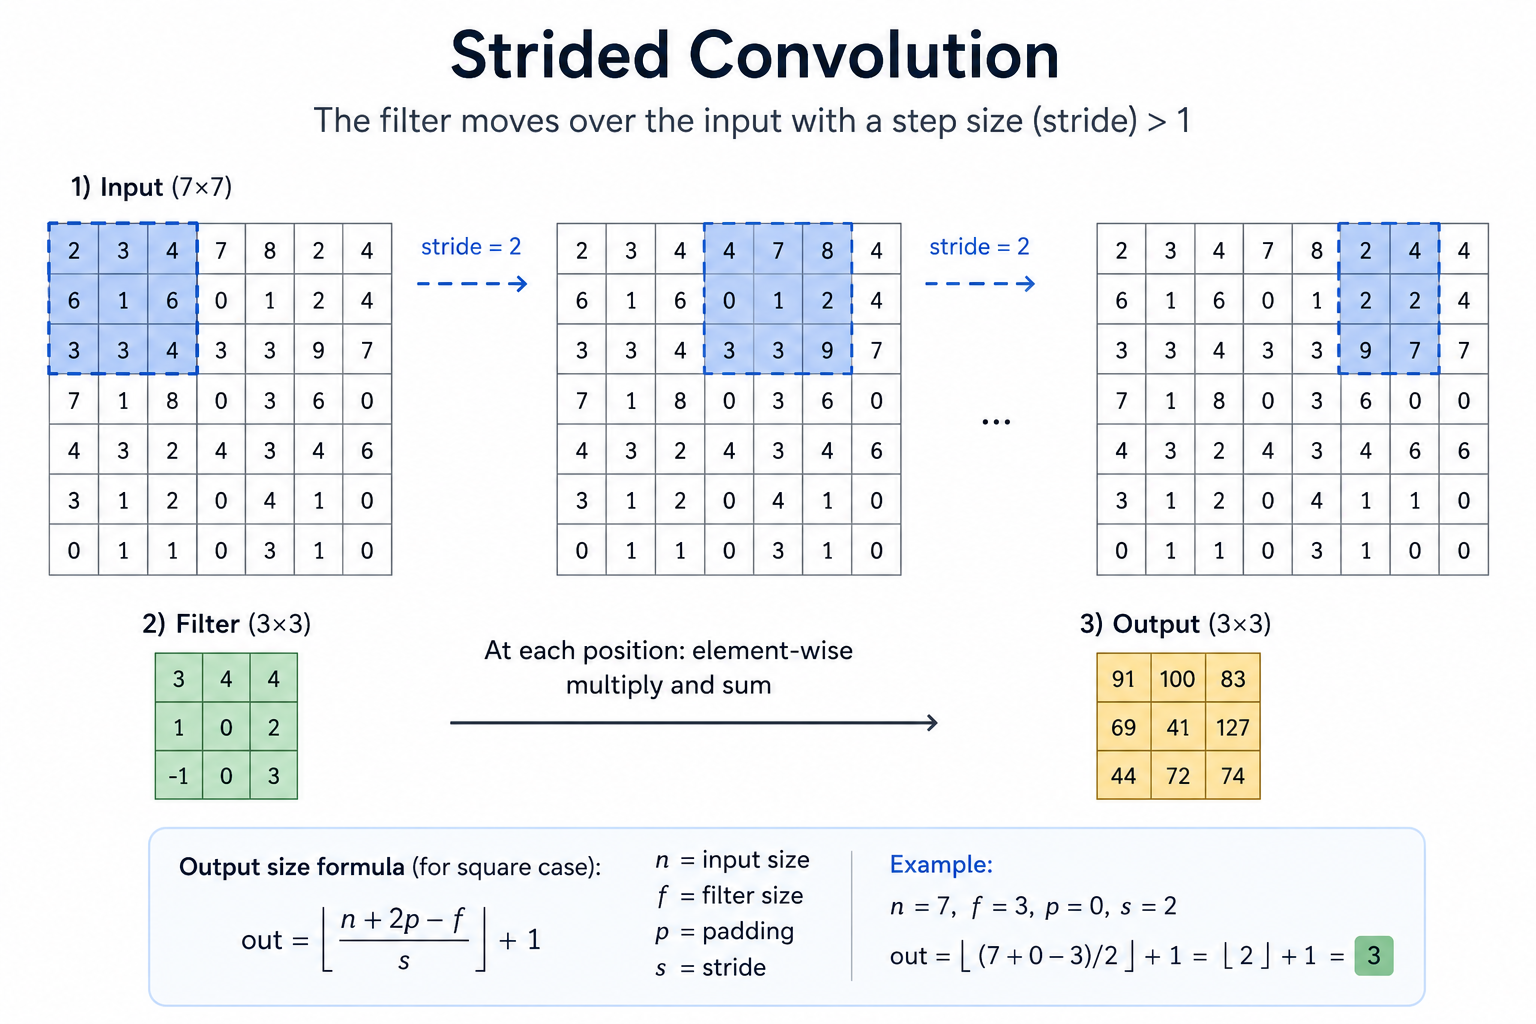
\includegraphics[width=0.8\linewidth]{images/stride.png}
    \caption{Stride}
    \label{fig:placeholder}
\end{figure}
\textbf{Technical Note: } Technically the convolution operator we have defined is known as cross-correlation in mathematics textbooks but for our purposes it doesn't really matter.
\subsection{Pooling}
Pooling is another operation which is used to reduced the size of the matrix while meaningfully capturing the information. This is similar to a sliding an imaginary square over the image and repeatedly either taking the max or taking the average of all the numbers in that square. The below figure shows it visually. 
\begin{figure}[H]
    \centering
    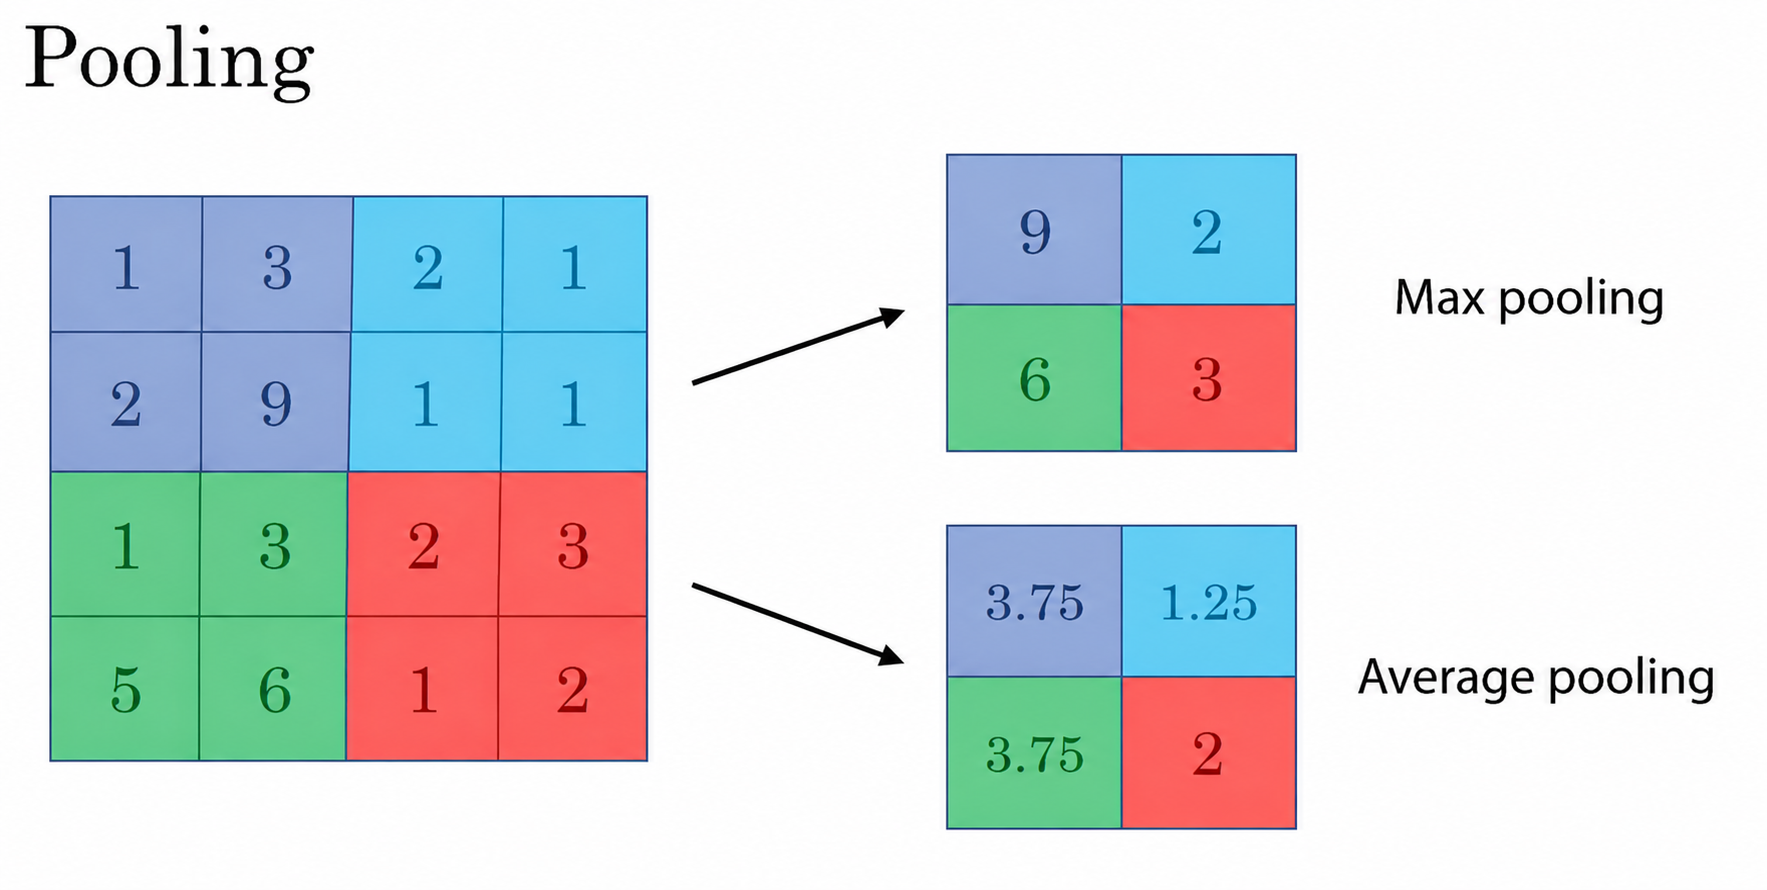
\includegraphics[width=0.5\linewidth]{images/pool.png}
    \caption{}
    \label{fig:placeholder}
\end{figure}
\subsection{CNN architechures}
These are the famous architechures built using varying various different values of hyperparameters(depth of the layer,max/average pooling multiple filters etc.) All of the architechures hold deep historical significance in the history of deep learning.
\subsubsection{LeNet}
\begin{figure}[H]
    \centering
    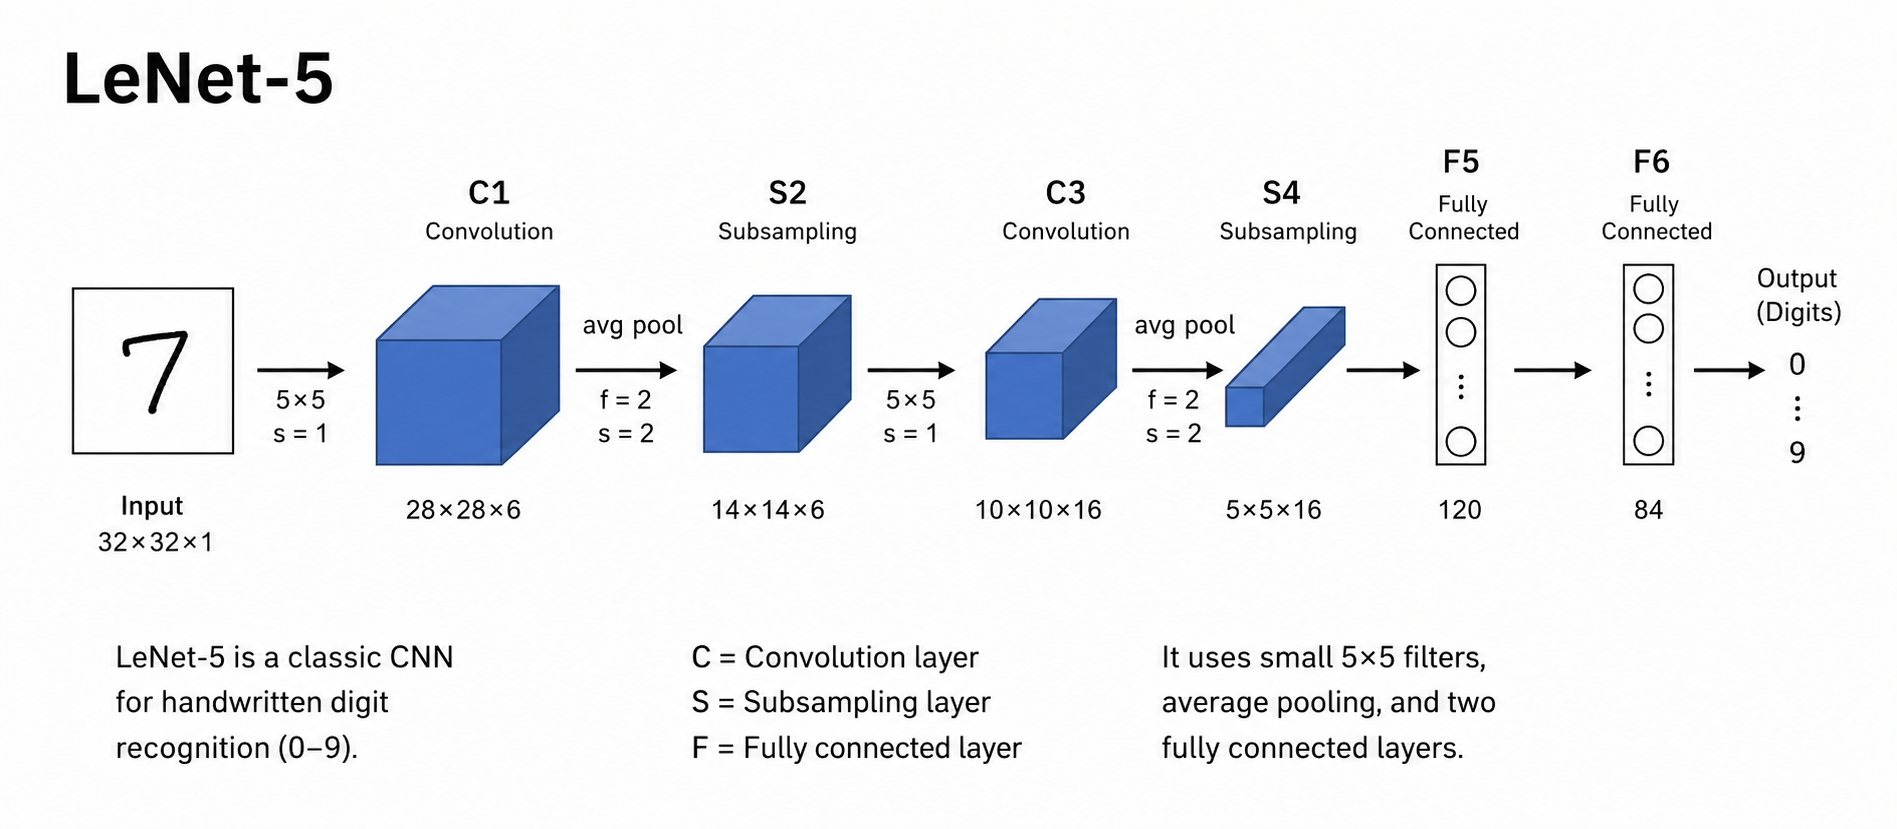
\includegraphics[width=1\linewidth]{images/lenet.png}
    \caption{LetNet Architechure}
    \label{fig:placeholder}
\end{figure}
\subsubsection{AlexNet}
\begin{figure}[H]
    \centering
    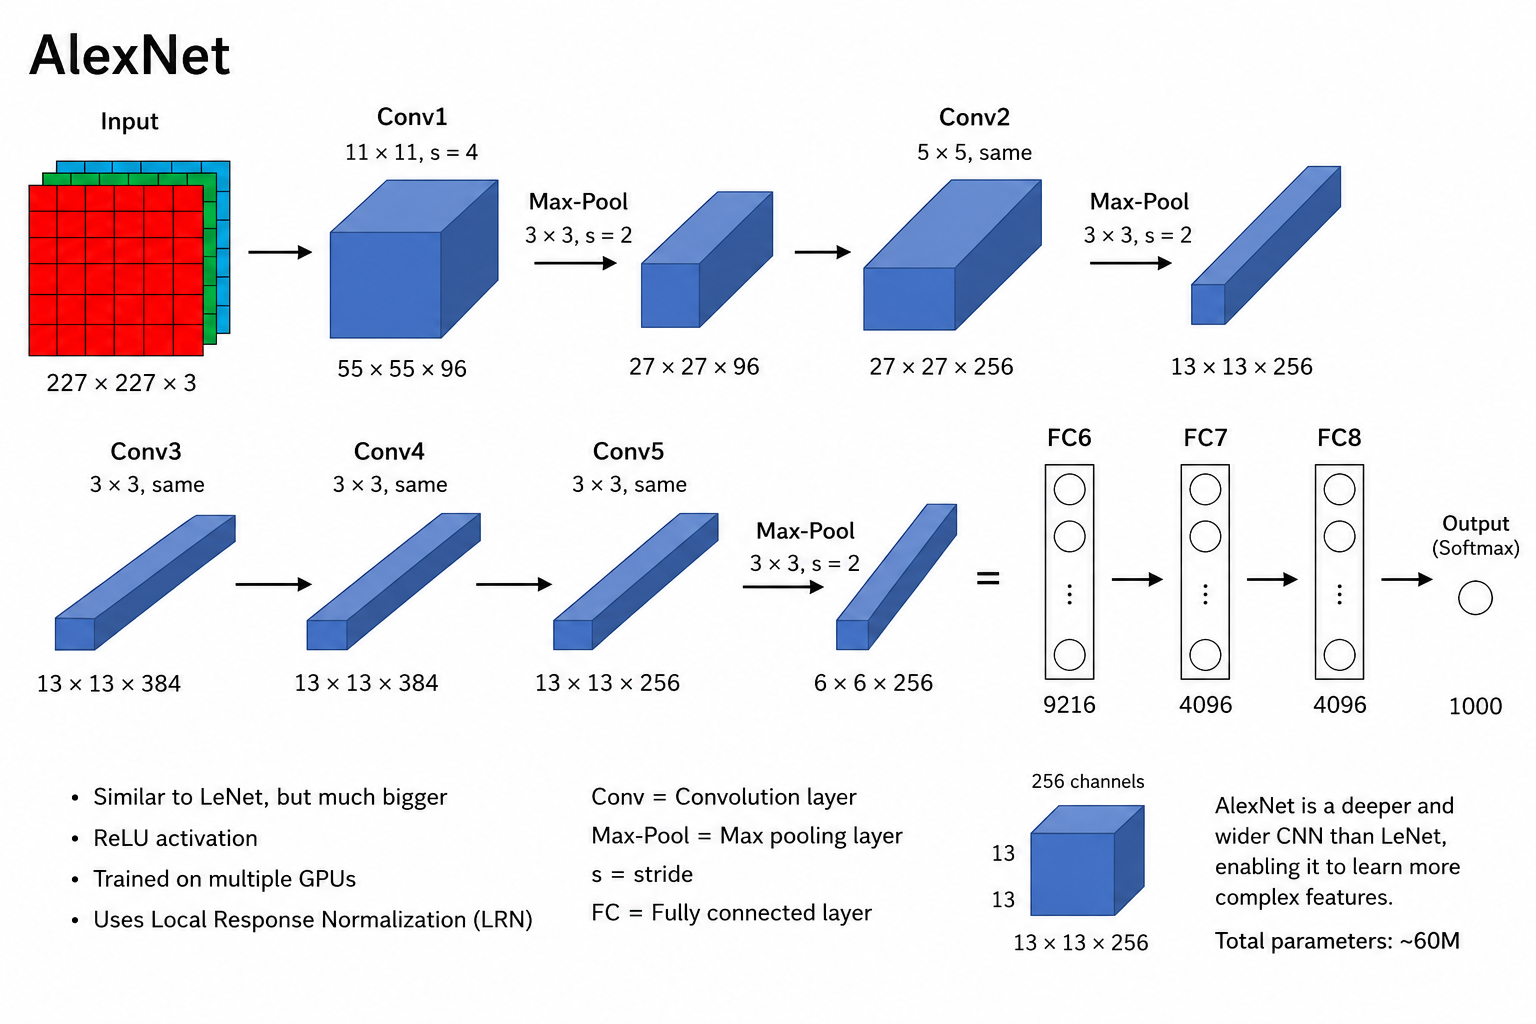
\includegraphics[width=\linewidth]{images/alexnet.png}
    \caption{AlexNet Architechure}
    \label{fig:placeholder}
\end{figure}
\subsubsection{VGG-16}
\begin{figure}[H]
    \centering
    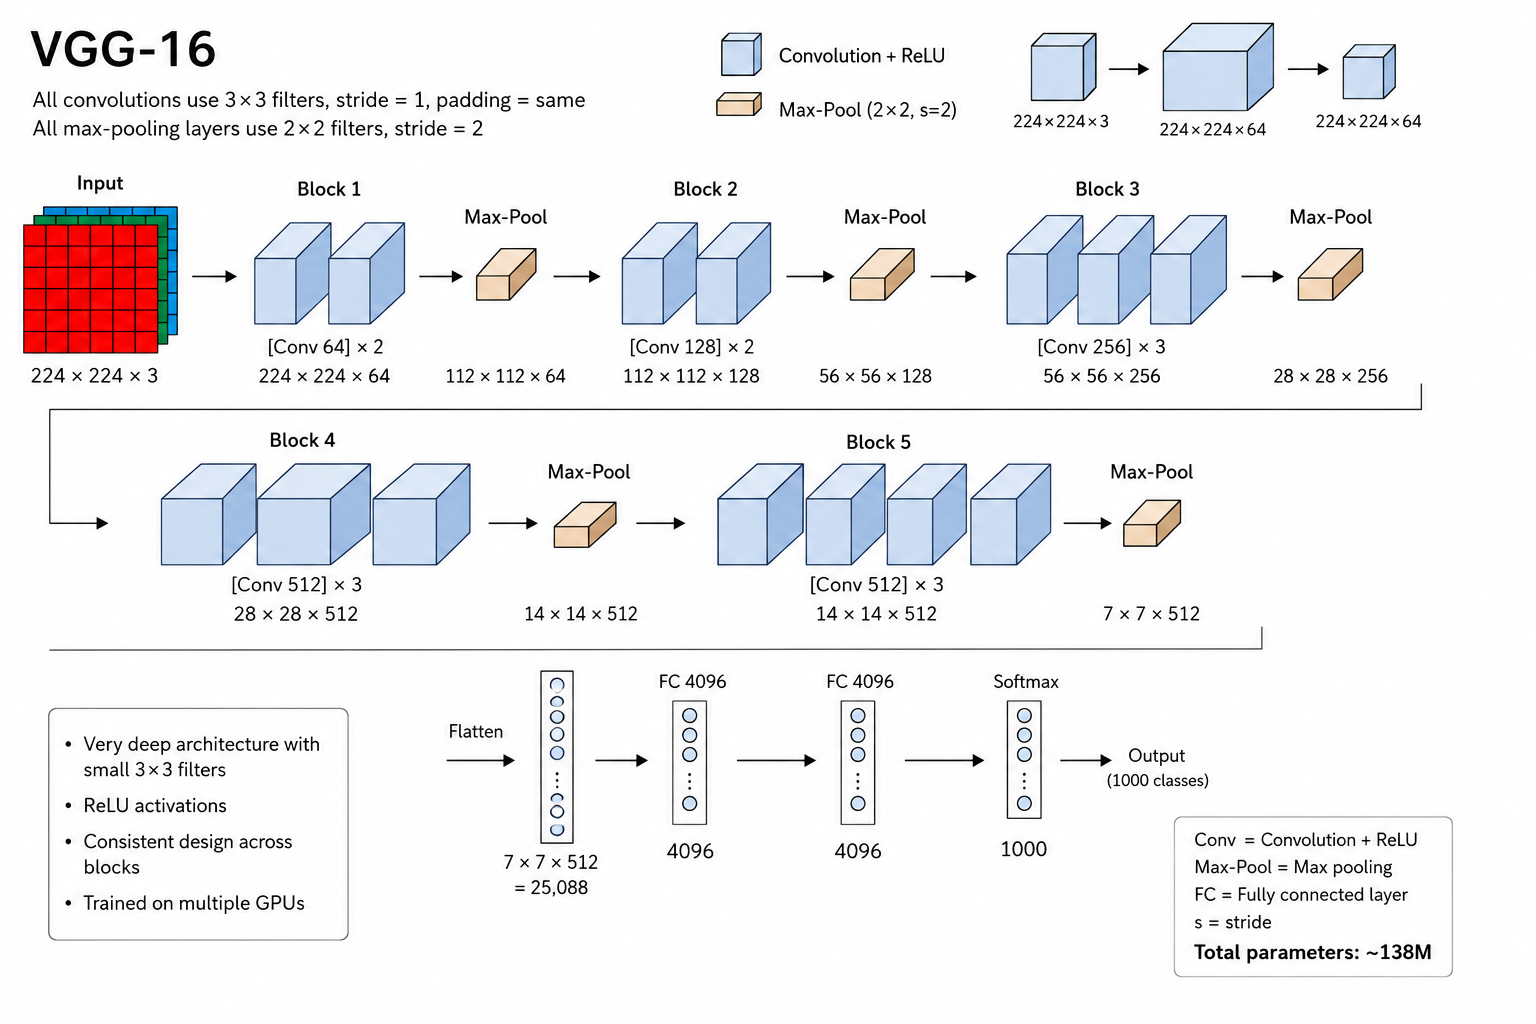
\includegraphics[width=\linewidth]{images/vgg.png}
    \caption{}
    \label{fig:placeholder}
\end{figure}
\subsubsection{ResNet}
In residual network(or ResNet for short) we apply some "skip connection" connections like shown in the image. 
\begin{figure}[H]
    \centering
    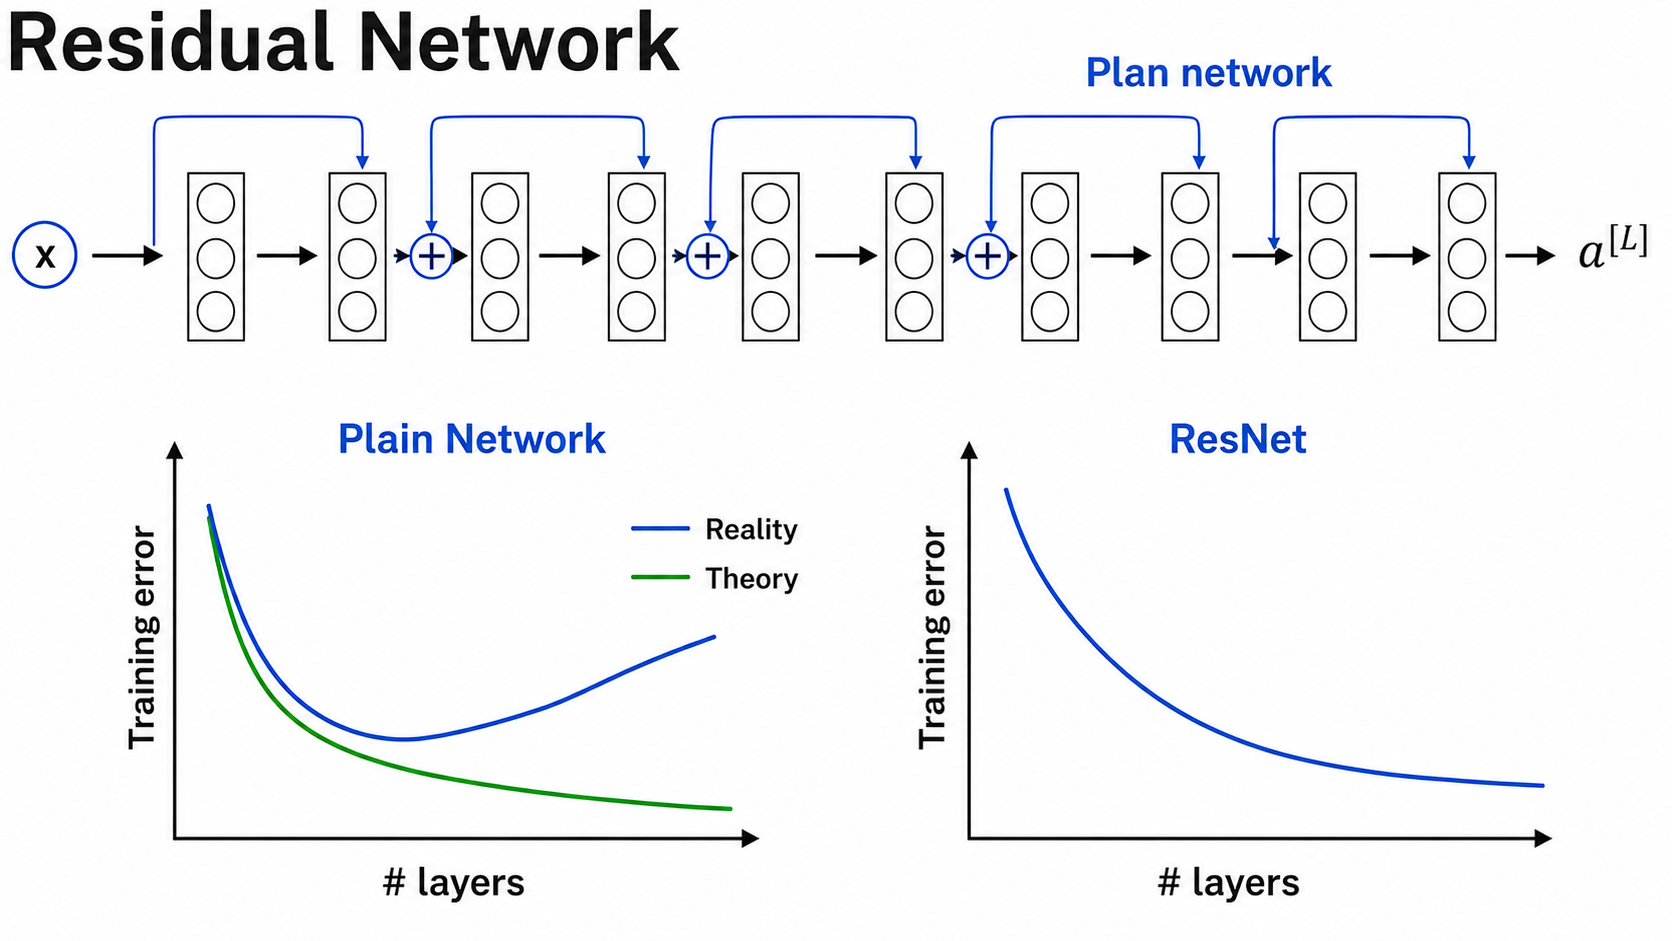
\includegraphics[width=0.5\linewidth]{images/res.png}
    \caption{}
    \label{fig:placeholder}
\end{figure}
In the paper [He et. al 2015] , the authors showed that residuals networks are much more efficient and powerful compared to other architechures. 
One inutition of why resnets work better is that as shown in the image, researchers found that on increasing the depth of the network sometimes even the training data error \textbf{increased}, this is quite suprising since a deep network should atleast be able to learn as much as the lesser depth network and learn the identity function for the rest. The real issue is that the neural network was unable to learn the identity function easily, this problem is solved in Resnets, because we do a "short cut"/"skip connection", our network is more easily able to learn the identity function.
\section{Mini tasks}
\subsection{Value class(Karpathy)}
Here I will use a simple binary classification on the iris dataset. I code it up using the MLP class.
\begin{lstlisting}
import random
from sklearn.datasets import load_iris

class Value:
    def __init__(self, data, _children=()):
        self.data = data
        self.grad = 0.0
        self._backward = lambda: None
        self._prev = set(_children)

    def __add__(self, other):
        other = other if isinstance(other, Value) else Value(other)
        out = Value(self.data + other.data, (self, other))

        def _backward():
            self.grad += out.grad
            other.grad += out.grad

        out._backward = _backward
        return out

    def __mul__(self, other):
        other = other if isinstance(other, Value) else Value(other)
        out = Value(self.data * other.data, (self, other))

        def _backward():
            self.grad += other.data * out.grad
            other.grad += self.data * out.grad

        out._backward = _backward
        return out

    def __pow__(self, power):
        out = Value(self.data ** power, (self,))

        def _backward():
            self.grad += power * (self.data ** (power - 1)) * out.grad

        out._backward = _backward
        return out

    def relu(self):
        out = Value(0 if self.data < 0 else self.data, (self,))

        def _backward():
            self.grad += (out.data > 0) * out.grad

        out._backward = _backward
        return out

    def backward(self):
        topo = []
        visited = set()

        def build_topo(v):
            if v not in visited:
                visited.add(v)

                for child in v._prev:
                    build_topo(child)

                topo.append(v)

        build_topo(self)

        self.grad = 1.0

        for node in reversed(topo):
            node._backward()

    def __neg__(self):
        return self * -1

    def __sub__(self, other):
        return self + (-other)

    def __radd__(self, other):
        return self + other

    def __rmul__(self, other):
        return self * other

    def __truediv__(self, other):
        return self * (other ** -1)


class Neuron:
    def __init__(self, nin, nonlin=True):
        self.w = [Value(random.uniform(-1, 1)) for _ in range(nin)]
        self.b = Value(0.0)
        self.nonlin = nonlin

    def __call__(self, x):
        act = sum((wi * xi for wi, xi in zip(self.w, x)), self.b)
        return act.relu() if self.nonlin else act

    def parameters(self):
        return self.w + [self.b]


class Layer:
    def __init__(self, nin, nout, nonlin=True):
        self.neurons = [Neuron(nin, nonlin=nonlin) for _ in range(nout)]

    def __call__(self, x):
        out = [n(x) for n in self.neurons]
        return out[0] if len(out) == 1 else out

    def parameters(self):
        return [p for neuron in self.neurons for p in neuron.parameters()]


class MLP:
    def __init__(self, nin, nouts):
        sizes = [nin] + nouts

        self.layers = [
            Layer(
                sizes[i],
                sizes[i + 1],
                nonlin=(i != len(nouts) - 1)
            )
            for i in range(len(nouts))
        ]

    def __call__(self, x):
        for layer in self.layers:
            x = layer(x)

        return x

    def parameters(self):
        return [p for layer in self.layers for p in layer.parameters()]


iris = load_iris()

X = iris.data[iris.target < 2]
y = iris.target[iris.target < 2]

random.seed(42)

mg_model = MLP(4, [4, 1])

print("Epoch  | Loss     | Bias Gradient")

for epoch in range(10):
    total_loss = Value(0.0)

    for xi, yi in zip(X, y):
        pred = mg_model([Value(float(x)) for x in xi])
        total_loss += (pred - yi) ** 2

    mg_loss = total_loss * (1.0 / len(X))

    for p in mg_model.parameters():
        p.grad = 0.0

    mg_loss.backward()

    mg_grad = mg_model.layers[1].neurons[0].b.grad

    for p in mg_model.parameters():
        p.data -= 0.05 * p.grad

    print(f"{epoch+1:<6} | {mg_loss.data:.4f} | {mg_grad:<.6f}")
\end{lstlisting}
\begin{table}[h]
\centering
\begin{tabular}{ccc}
\hline
Epoch & Loss & Bias Gradient \\
\hline
1  & 0.3349 & 0.884352 \\
2  & 0.7557 & -1.389760 \\
3  & 1.5380 & 2.412193 \\
4  & 1.7987 & -2.392820 \\
5  & 0.2881 & -0.554322 \\
6  & 0.2094 & -0.265331 \\
7  & 0.1759 & -0.043725 \\
8  & 0.1660 & 0.065513 \\
9  & 0.1607 & 0.099752 \\
10 & 0.1558 & 0.108238 \\
\hline
\end{tabular}
\caption{}
\label{tab:micrograd_training}
\end{table}
\subsection{Building a simple MNIST classifier}
This is famously called the "Hello world" of neural networks. I have implemented a simple Neural network with one hidden layer in pytorch. I have used the relu activation function and adam's optimizer.
\begin{lstlisting}
import torch
import torch.nn as nn
import torch.optim as optim
from torchvision import datasets, transforms
from torch.utils.data import DataLoader

transform = transforms.ToTensor()

train_loader = DataLoader(datasets.MNIST('data', train=True, download=True, transform=transform), batch_size=64, shuffle=True)
test_loader = DataLoader(datasets.MNIST('data', train=False, transform=transform), batch_size=1000, shuffle=False)

class NN(nn.Module):
    def __init__(self):
        super().__init__()
        self.fc1 = nn.Linear(784, 32)
        self.fc2 = nn.Linear(32, 10)

    def forward(self, x):
        x = x.view(-1, 784)
        x = torch.relu(self.fc1(x))
        return self.fc2(x)

model = NN()
optimizer = optim.Adam(model.parameters(), lr=0.01)
criterion = nn.CrossEntropyLoss()

for epoch in range(3):
    model.train()
    for data, targets in train_loader:
        optimizer.zero_grad()
        loss = criterion(model(data), targets)
        loss.backward()
        optimizer.step()
        
    model.eval()
    correct = 0
    with torch.no_grad():
        for data, targets in test_loader:
            outputs = model(data)
            correct += outputs.argmax(dim=1).eq(targets).sum().item()
            
    print(f"Epoch {epoch+1} | Accuracy: {100. * correct / len(test_loader.dataset):.2f}%")
\end{lstlisting}
This achieves an accuracy of 95.54\%. 
\section{Week 5}
\subsection{Transfer Learning}

Suppose we have a huge neural network already pretrained on a huge amount of speech recognition data. Now say I want it to very strongly recognize a "wake word" like "Alexa"(the word that wakes up Alexa). Instead of training a whole new network from scratch, I can take this pretrained network, block/freeze the earlier layers, and only fine tune the later layers so the network reacts more strongly to this particular word.

This kind of fine tuning works well when:
\begin{enumerate}
    \item Task A and Task B have the same input $x$.
    \item We have a lot more data for Task A than Task B.
    \item Low level features learned from Task A could be helpful for learning Task B.
\end{enumerate}


\subsection{Data Augmentation}

More data almost always helps, but collecting new data is expensive. Data augmentation is a cheap way around this, we generate new but realistic training examples out of the ones we already have. In computer vision(say we're building a cat detector), some common techniques are:
\begin{itemize}
    \item Random crops
    \item Flipping(horizontal, sometimes vertical)
    \item Shearing
    \item Rotation
    \item color shifting
\end{itemize}
A cat is still a cat if you crop it, flip it, or rotate it slightly, so these transformations let the model see more "versions" of the same image without us collecting a single new photo.

\subsection{Representation Learning}

One interesting thing about Convolutional Neural Networks is that they automatically learn useful representations of the image. We never explicitly tell the network to detect edges, colours or shapes. All we tell it is to minimize the loss function, yet these features naturally emerge during training.

The following figures show what different layers of a CNN are learning. The initial layers mainly detect very simple features such as edges, corners, gradients and colours. These simple features are then combined by the deeper layers to recognize textures and object parts. As we move even deeper into the network, these features are combined further to recognize complete objects. In other words, every layer builds on the features learned by the previous layer.

This also gives us an intuition as to why transfer learning works so well. Low level features such as edges, colours and simple textures are useful for almost every computer vision task. Hence the earlier layers of a pretrained network are already doing a very good job. We only need to retrain the last few layers so that they learn features specific to our new task.
\section{Week 6}

\subsection{Recurrent Neural Networks (RNN)}

So far all the neural networks we have studied assume that every input sample is independent of every other sample. This assumption works perfectly for tasks such as image classification where every image can be processed separately. However, many real world problems involve sequential data where the previous inputs play a very important role in predicting the current output.

Consider the sentence

\begin{center}
\textit{The clouds are dark, it will probably \_\_\_\_.}
\end{center}

Even without seeing the last word, it is fairly easy to predict that the missing word could be \textit{rain}. This prediction is only possible because we have access to the previous words. A traditional neural network has no mechanism to remember this information, which is why we need for Recurrent Neural Networks (RNNs).

The key idea behind an RNN is remarkably simple. Instead of discarding all information after processing one input, the network maintains a hidden state which acts as a memory. This hidden state is continuously updated as new inputs arrive, allowing information from previous time steps to influence future predictions.

Suppose the input sequence is

\[
x^{\langle1\rangle},x^{\langle2\rangle},\ldots,x^{\langle T\rangle}.
\]

At every time step the hidden state is updated using

\[
a^{\langle t\rangle}
=
g
\left(
W_{aa}a^{\langle t-1\rangle}
+
W_{ax}x^{\langle t\rangle}
+
b_a
\right),
\]

where $g$ is usually chosen as $\tanh$. The prediction at every time step is then computed as

\[
\hat y^{\langle t\rangle}
=
g
\left(
W_{ya}a^{\langle t\rangle}
+
b_y
\right).
\]

One important observation is that the weight matrices remain exactly the same at every time step. We are not learning a new neural network for every word in the sequence. Instead, the same parameters are reused repeatedly which allows an RNN to process sequences of arbitrary length while keeping the number of learnable parameters fixed.

Although RNNs perform much better than feedforward networks on sequential data, they suffer from one major drawback. As the sequence becomes longer, the network gradually loses information from the earlier time steps. This makes it difficult to capture long term dependencies, a problem which we will address later using LSTMs and GRUs.
\begin{figure}[H]
    \centering
    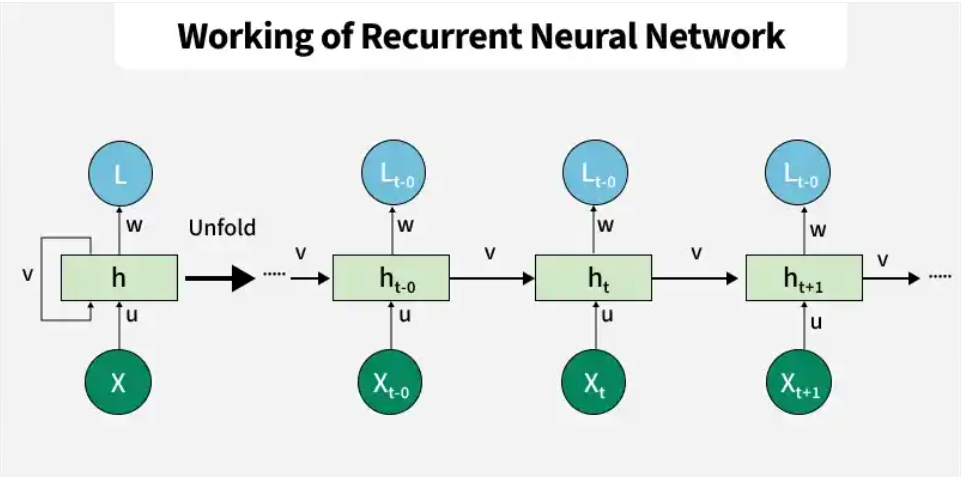
\includegraphics[width=0.5\linewidth]{images/rnn.png}
    \caption{Caption}
    \label{fig:placeholder}
\end{figure}
\subsection{Backpropagation Through Time (BPTT)}

Training an RNN is conceptually very similar to training any other neural network. The only difference is that every hidden state depends on the hidden state from the previous time step. Consequently, the loss at the current time step indirectly depends on all previous hidden states as well.

To compute the gradients, we first unroll the RNN across all time steps. After unrolling, the network resembles a very deep feedforward neural network where each layer corresponds to one time step. Since all these layers share the same parameters, the gradients computed from every time step are accumulated before updating the weights. This entire procedure is known as \textbf{Backpropagation Through Time (BPTT).}

The total loss over a sequence is generally written as

\[
L
=
\sum_{t=1}^{T}
L^{\langle t\rangle},
\]

where $L^{\langle t\rangle}$ denotes the loss corresponding to the prediction at time step $t$.

One major challenge while performing BPTT is the vanishing and exploding gradient problem. During backpropagation the gradients are repeatedly multiplied while travelling through many time steps. If these values become very small, the network almost stops learning information from the distant past. This is known as the vanishing gradient problem. On the other hand, if they become excessively large, the optimization process becomes unstable, resulting in exploding gradients.

Gradient clipping is often used to handle exploding gradients, while entirely new recurrent architectures such as LSTMs and GRUs were introduced to address the vanishing gradient problem.

\subsection{Long Short-Term Memory (LSTM) and Gated Recurrent Units (GRU)}

As discussed in the previous subsection, vanilla RNNs suffer from the vanishing gradient problem, making it difficult for them to retain information over long sequences. Consequently, they often fail to capture long term dependencies present in sequential data. To overcome this limitation, more sophisticated recurrent architectures such as Long Short-Term Memory (LSTM) networks and Gated Recurrent Units (GRUs) were introduced.

The central idea behind both these architectures is the use of gates. Rather than updating the hidden state blindly at every time step, the network learns what information should be remembered, what should be discarded and what should be passed to the next time step. This allows the network to selectively preserve useful information while eliminating irrelevant details.

An LSTM introduces a separate cell state $C_t$ which acts as the long term memory of the network. Information flows through this cell state with only minor modifications at every time step, making it much easier to preserve important information across long sequences. Three different gates control this flow of information namely the forget gate, input gate and output gate.

The forget gate determines how much of the previous cell state should be retained and is computed as

\[
f_t=\sigma(W_f[h_{t-1},x_t]+b_f),
\]

where $\sigma$ denotes the sigmoid activation function. Values close to $1$ indicate that the information should be retained, while values close to $0$ imply that it should be discarded.

The input gate decides what new information should be stored in the memory,

\[
i_t=\sigma(W_i[h_{t-1},x_t]+b_i),
\]

while a candidate memory state is generated as

\[
\tilde{C}_t=\tanh(W_c[h_{t-1},x_t]+b_c).
\]

Using these quantities, the cell state is updated according to

\[
C_t=f_t C_{t-1}+i_t\tilde{C}_t,
\]

where $\odot$ denotes element-wise multiplication.

Finally, the output gate controls what information is passed to the next hidden state,

\[
o_t=\sigma(W_o[h_{t-1},x_t]+b_o),
\]

and the hidden state is computed as

\[
h_t=o_t\tanh(C_t).
\]

Although these equations may appear intimidating at first glance, the intuition behind them is fairly simple. The forget gate removes unnecessary information, the input gate stores useful new information, while the output gate decides what information should be exposed to the next layer. This gating mechanism enables LSTMs to retain information over significantly longer sequences compared to vanilla RNNs.
\begin{figure}[H]
    \centering
    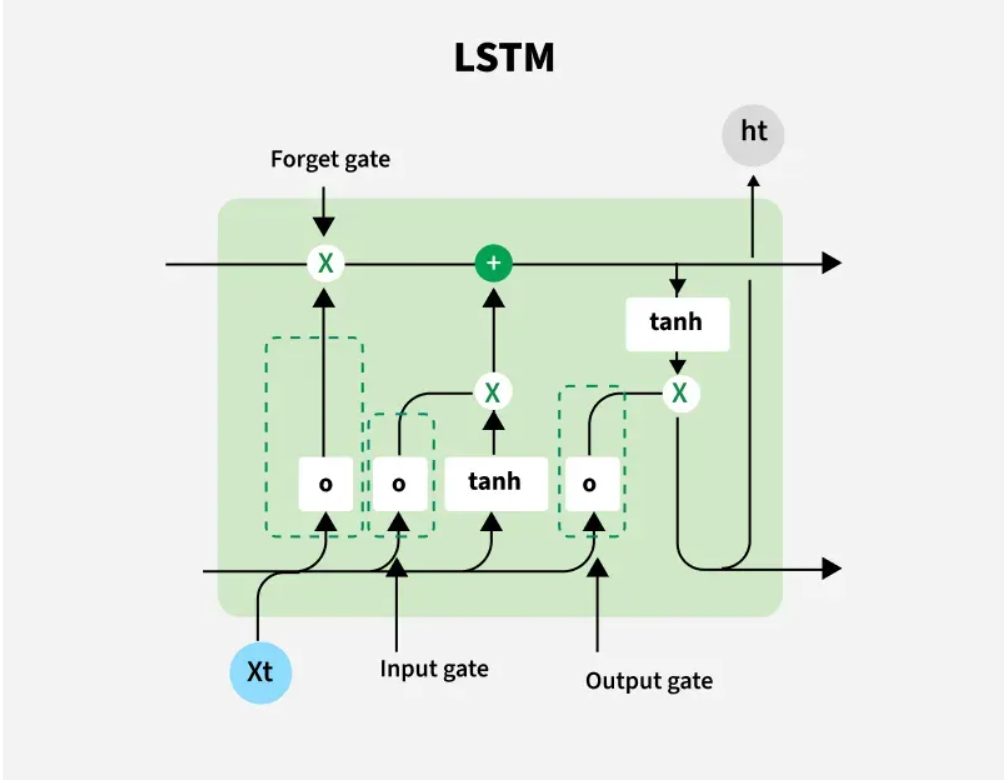
\includegraphics[width=0.5\linewidth]{images/lstm.png}
    \caption{Caption}
    \label{fig:placeholder}
\end{figure}
Gated Recurrent Units (GRUs) were later proposed as a simpler alternative to LSTMs. Instead of maintaining a separate cell state and three different gates, a GRU combines these ideas into a more compact architecture with only two gates namely the update gate and the reset gate. This considerably reduces the number of learnable parameters while still preserving the ability to model long term dependencies.

The update gate is given by

\[
z_t=\sigma(W_z[h_{t-1},x_t]+b_z),
\]

while the reset gate is computed as

\[
r_t=\sigma(W_r[h_{t-1},x_t]+b_r).
\]

The reset gate is then used to generate a candidate hidden state,

\[
\tilde{h}_t=
\tanh\left(
W_h[r_t h_{t-1},x_t]+b_h
\right),
\]

and the final hidden state is updated according to

\[
h_t=(1-z_t) h_{t-1}+z_t\tilde{h}_t.
\]

The update gate determines how much of the previous hidden state should be preserved, while the reset gate controls how much past information should be ignored while computing the candidate hidden state. Despite being considerably simpler than an LSTM, GRUs often achieve very similar performance while requiring fewer parameters and lower computational cost.
\begin{figure}[H]
    \centering
    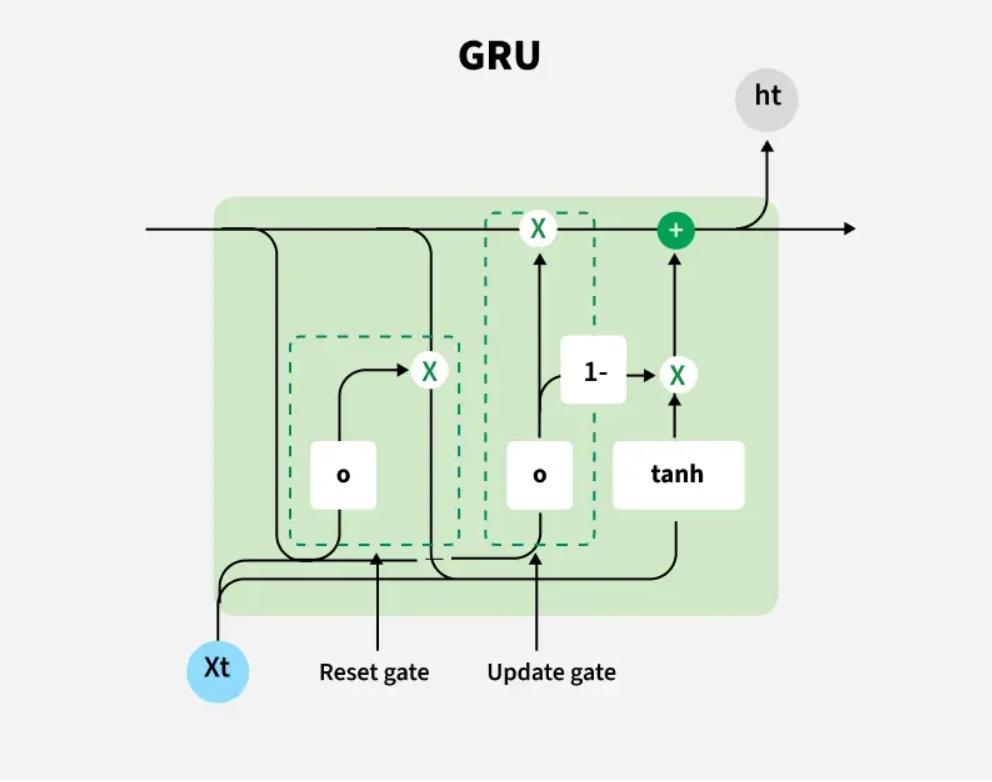
\includegraphics[width=0.5\linewidth]{images/gru.png}
    \caption{Caption}
    \label{fig:placeholder}
\end{figure}
In practice, both LSTMs and GRUs have largely replaced vanilla RNNs whenever long sequential dependencies are involved. They have been successfully applied to problems such as machine translation, speech recognition, sentiment analysis and time series forecasting.

\subsection{Character-Level Language Modelling}

This is the same character level generation idea Karpathy uses to generate baby names in makemore. It's a vanilla RNN(Week 6) trained to predict the next character given all the previous ones, one character at a time. Once trained, we sample from it repeatedly, feeding each generated character back in as the next input(exactly like the inference loop in the GPT section below), until it hits a stop token or the max length.

% TODO: paste your generated dinosaur names / loss curve here


\section{Week 7}

\subsection{Attention: Motivation}

So far we were using sequence to sequence models with an encoder and decoders. There is a technique called \textit{attention} which makes these models even better. The attention idea has been one of the most influential ideas in deep learning.

Suppose we are trying to translate a long sentence from French to English. The way we have been building our models, it converts the whole sentence into a vector first and then tries to decode it. This reduces the efficiency if the sentence is long. In reality humans don't do this either. If a human would translate this sentence, he/she wouldn't read the whole sentence and memorize it then try to translate it. He/she translates a part at a time. We will discuss the attention model that works like a human, that looks at parts at a time. This significantly increases the accuracy even with longer sequences.

At first the attention model was developed for machine translation, but then other applications used it like computer vision, and it eventually led to a whole new family of architectures. The attention model was described in this paper: [Bahdanau et al., 2014. Neural Machine Translation by Jointly Learning to Align and Translate]

\subsection{Query, Key, Value}

So now the question is, how does the model actually decide which part of the input to "look at" at any given moment? This is where Query, Key and Value come in, and honestly the easiest way to think about it is like a search engine.

Say you type something into a search bar, that's your \textbf{Query}, what you're looking for. Every document on the internet has some \textbf{Key}, a short description of what it's about, which gets compared against your query. Whichever documents have keys that match your query well, you get their \textbf{Value}, the actual content.

Attention works the exact same way. Every word in our sentence gets turned into three vectors, a query, a key and a value, by multiplying with learned weight matrices:
$$Q = XW_q, \qquad K = XW_k, \qquad V = XW_v$$
When a word generates its query, it's basically asking "who in this sentence is relevant to me right now". Every other word offers up its key to answer that, and whichever ones match well, we pull in their value.

When $Q,K,V$ all come from the same sentence $X$, we call this \textbf{self-attention}, i.e. the sentence is attending to itself.

\subsection{Scaled Dot-Product Attention}

Now we need a way to actually measure "how well does this query match this key". The simplest way to measure similarity between two vectors is a dot product, so that's what we use, $QK^T$. The bigger this number, the more the query and key agree, the more attention that word deserves.

There's one catch though. When the vectors are high dimensional, this dot product can get really large, which pushes the softmax we're about to apply into a region where it basically becomes one-hot(all the attention collapses onto a single word, gradients vanish everywhere else). To fix this we scale down by $\sqrt{d_k}$ before doing anything else.

Once we have these scaled scores, we softmax them so they turn into proper weights summing to 1, and use them to take a weighted average of the value vectors:
$$\text{Attention}(Q,K,V) = \text{softmax}\left(\frac{QK^T}{\sqrt{d_k}}\right)V$$
This one line is basically the entire mechanism, score how relevant each word is, normalize the scores, mix the values accordingly.

\subsection{Multi-Head Attention}

Here's a problem with just having a single $Q,K,V$: a sentence has many different kinds of relationships between its words at once, grammar, meaning, tone. One single attention "head" can really only latch onto one type of relationship at a time.

So instead we run several heads in parallel, each with its own separate $W_q, W_k, W_v$ matrices, and let each head specialize in whatever relationship it finds useful. We then concatenate all their outputs and pass it through one more linear layer to mix everything back together:
$$\text{MultiHead}(Q,K,V) = \text{Concat}(head_1,\dots,head_h)\,W_O$$

\subsection{Positional Encoding}

Here's something interesting, self-attention on its own has no idea what order the words came in! If you scrambled the sentence, attention would compute the exact same weights, just scrambled the same way (this is called being permutation invariant). Obviously word order matters a lot, "dog bites man" and "man bites dog" mean very different things.

So we manually inject position information into every word before running attention, by adding a positional vector built out of sines and cosines of different frequencies:
$$p(t) = [\sin(w_1t), \cos(w_1t), \dots], \qquad w_k = \frac{1}{10000^{2k/d}}$$
Using multiple frequencies like this gives every position a unique fingerprint (kind of like a fancy binary encoding of position), and it generalizes to sequences longer than anything seen in training.

\subsection{Transformer Architecture}

This is the big one, introduced in \textit{Attention Is All You Need}(Vaswani et al. 2017). The core idea is: why do we even need recurrence anymore? RNNs process one word at a time because each hidden state depends on the previous one, this is slow to train and struggles with long range dependencies. If attention alone can figure out which words are relevant to which, we can throw away recurrence entirely.

The \textbf{encoder} takes the input sentence, adds positional encoding (since plain attention doesn't know word order), and passes it through a stack of $N$ identical blocks. Each block does multi-head self attention, then a residual connection and layer norm, then a small feedforward MLP, then another residual connection and layer norm.

The \textbf{decoder} looks almost identical, but with two differences. First, its self attention is \textbf{masked}, future words are hidden (set to $-\infty$ before the softmax) so the model can't cheat by peeking ahead while generating. Second, it has an extra attention layer right after, where the Query comes from the decoder but the Key and Value come from the encoder's output, this is exactly how the decoder "looks back" at the original sentence while generating, just like our attention model from the very first section!

Finally, the decoder's output goes through one linear layer and a softmax over the vocabulary to predict the next word.

\section{Week 8}
All the models were implemented in a very basic fashion. The transformer was made following the official keras tutorial \url{https://keras.io/examples/nlp/text_classification_with_transformer/}. It is coded up in the notebook inside the Project folder. 

The github repo link is here: {https://github.com/OPboi05/Summer-of-Science-Neural-Networks.git}

\printbibliography
\end{document}